
\section{Abstract}
The nicotinic acetylcholine receptor (nAChR) and other pentameric ligand-gated ion channels (pLGICs) are native to neuronal membranes with an unusual lipid composition. While it is well-established that these receptors can be significantly modulated by lipids, the underlying mechanisms have been primarily studied in model membranes with only a few lipid species. Here we use coarse-grained molecular dynamics (MD) simulation to probe specific binding of lipids in a complex quasi-neuronal membrane. We ran a total of 50 microseconds of simulations of a single nAChR in a membrane composed of 36 species of lipids. Competition between multiple lipid species produces a complex distribution. We find that overall, cholesterol selects for concave intersubunit sites and PUFAs select for convex M4 sites, while monounsaturated and saturated lipids are unenriched in the nAChR boundary. In order to characterize binding to specific sites, we present a novel approach for calculating a ``density-threshold affinity'' from continuous density distributions. We find that affinity for M4 weakens with chain rigidity, which suggests flexible chains may help relax packing defects caused by the conical protein shape. For any site, PE headgroups have the strongest affinity of all phospholipid headgroups, but anionic lipids still yield moderately high affinities for the M4 sites as expected.  We observe cooperative effects between anionic headgroups and saturated chains at the M4 site in the inner leaflet. We also analyze affinities for individual anionic headgroups. Combined, these insights may reconcile several apparently contradictory experiments on the role of anionic phospholipids in modulating nAChR.
%The nicotinic acetylcholine receptor (\nachr ) and other pentameric ligand-gated ion channels (\plgic s) are native to complex neuronal membranes with an unusual lipid composition. While it is well-established that these receptors can be significantly modulated by lipids, the underlying mechanisms have been primarily studied in model membranes with only a few lipid species.  Here we use coarse-grained molecular dynamics (MD) simulation to test whether specific binding sites observed within model membranes are recovered for a complex quasi-neuronal membrane. We ran a total of 50 microseconds of simulations of a single \nachr{} in a membrane composed of 36 species of lipids. %, including heteroacidic and homoacidic lipids, multiple chain lengths and unsaturation sites, multiple neutral and anionic phospholipid headgroups, and cholesterol.   at the concave intersubunit interfaces as well as convex sites around the M4 helix
% Competition between multiple lipid species produces a complex distribution. We find that overall, cholesterol selects for concave intersubunit sites and PUFAs select for convex M4 sites, while monounsaturated and saturated lipids are unenriched in the \nachr{} boundary. %While those results are consistent with our previous observations from model membranes,  
% In order to characterize binding to specific sites, we present a novel approach for calculating a ``\newaffinity'' from continuous density distributions. The \newaffinities{} reveal a monotonic weakening of affinity with acyl chain rigidity, which is consistent with our previous hypothesis that flexible chains are important for relaxing the packing defects caused by the conical star-shaped \nachr{}.
%We observe that cholesterol selects for intersubunit sites , as expected from model membranes, but has a relatively strong affinity for M4 sites as well. Conversely, neutral n-3 PUFAs are most favorable at M4 sites as expected,  but also successfully competed with cholesterol and saturated lipids for intersubunit sites. 
%For any site, PE headgroups have the strongest affinity of all phospholipid headgroups, but anionic lipids still yield moderately high affinities for the M4 sites as expected. Interestingly, we observe cooperative effects between anionic headgroups and saturated chains at the M4 site in the inner leaflet.  Combined, these insights may reconcile several apparently contradictory experiments on the role of anionic phospholipids in modulating \nachr.     % In model membranes \nachr~is functionally dependent on cholesterol and are modulated by anionic lipids. We showed previously that 1) \nachr~preferentially interacts with long acyl-chained and highly unsaturated polyunsaturated fatty acids (PUFAs) over shorter chained and less saturated PUFAs. 2) \plgic~inter-subunit and M4 have lipid specificity for raft forming lipids and PUFAs, respectively, with anionic lipids favoring sites with more cationic amino acids.  \nachr~boundary lipids in a native neuronal membrane are unknown. Using coarse grained molecular dynamics we simulate \nachr~embedded in a neuronal phospholipid membrane and analyze boundary lipids distribution and using a new approach for calculating binding affinities ($\Delta G$) predict \nachr~neuronal boundary lipid distributions. Cholesterol and neutral n-3 PUFAs had the strongest occupancy affinities of lipids simulated but had the strongest affinities for inter-subunit and M4 sites respectively. Anionic lipids were energetically unfavorable at the TMD in the outer leaflet but had the strongest affinities for inner M4 sites independent of acyl-chain or head group size. 
%We hypothesize lipid-protein occupancy sites where 1) PUFAs, and raft forming lipids would occupy around the M4 and inter-subunit sites respectively. 2) anionic lipids would occupy an inter-subunit region of \nachr~ in the inner leaflet. We analyze 20 potential lipid-protein occupancy sites through $\Delta G$ free energy calculations.

%\begin{keyword}
%%% keywords here, in the form: keyword \sep keyword
%%Jake the Dog \sep Finn the Human
%Neuron \sep \nachr \sep pLGIC \sep PUFAs \sep Cholesterol \sep Ion Channel \sep DHA \sep Affinity Calculation
%%% MSC codes here, in the form: \MSC code \sep code
%%% or \MSC[2008] code \sep code (2000 is the default)
%
%\end{keyword}
%\end{frontmatter}

%%
%% Start line numbering here if you want
%%

%% main text
\section{Introduction}
\label{Intro}

The nicotinic acetylcholine receptor (\nachr)~is a well studied excitatory pentameric ligand gated ion channel (\plgic s). \nachr s are found at high density in post-synaptic membranes and the neuromuscular junction in mammals, and the electric organ in \textit{Torpedo} electric rays. The \nachr~is activated by the binding of agonists such as nicotine or acetylcholine to the orthosteric site in the extra-cellular domain (ECD). When post-synaptic \nachr s are activated {\it en-mass} they stimulate an action potential. Thus \nachr s~play a critical role in both cognition and memory\cite{Henault2015} and neuromuscular function \cite{Mukhtasimova2016,Kalamida2007}. \nachr~ and the greater \plgic~superfamily play various roles in neurological diseases related to inflammation \cite{Taly2009,Patel2017,Yocum2017,Egea2015},  addiction \cite{Cornelison2016}, chronic pain \cite{Xiong2012}, Alzheimer's Disease \cite{Walstab2010,Picciotto_Neuroprotection_2008,MartinRuiz_4_1999,Kalamida2007},spinal muscular atrophy \cite{Arnold_Reduced_2004}, schizophrenia \cite{Haydar2010,Kalamida2007} and neurological autoimmune diseases \cite{Lennon_Immunization_2003, Kumari2008}.
%Egea2015

\nachr s~are highly sensitive to their local lipid environment. \nachr~ poorly conducts ions in model phosphatidylcholine (PC)-only membranes, but can conduct a current with the addition of cholesterol or anionic lipids \cite{Baenziger2017,Dalziel1980,Ellena1983,M.CriadoH.Eibl1982,Fong1986,Fong1987,Jones1988,Sunshine1994,DaCosta2009b,Baenziger2017}, though too much  cholesterol can also cause a loss of function \cite{M.CriadoH.Eibl1982,Mantipragada2003,Barrantes2010a,Baier2011a}. %Barrantes2014
%\grace{LMS There are more examples of this, check Barrantes papers from aughts}  
Functional studies using \xo~ \cite{Zhou2003,Gamba2005,Chen2015,Kouvatsos2016,Nys2016,Polovinkin2018,Moffett2019,Kumar2020} require lipid additives such as asolectin\cite{M.CriadoH.Eibl1982,Zhou2003,Gamba2005,Chen2015,Nys2016,Polovinkin2018,Moffett2019,Kumar2020} or lipids from synaptic membranes \cite{Conti2013} to recover native levels of \nachr{} ion flux.  %This suggests 1) \nachr{} requires more than lipid diversity for native function, and 2) \nachr{} has specific boundary lipids required for native function not found in \xo or there are not enough of these specific lipids to play a boundary role.  
Understanding the mechanism of modulation requires understanding how and where the modulating lipid interacts with the receptor, and these interactions may themselves be dependent upon the rest of the lipid composition.  
%\grace{LMS we don't know the boundary composition, at all, remember? Please unpack/fix this sentence like you did for similar sentences in your thesis.} %lipid composition are essential to function in model membranes or its native neuronal membranes.%Why using addition membranes to restore function rather than cholesterol or anionic lipids is unclear \liam{not quite}. 

Mammalian neuronal membranes \cite{Isolated1969, Taguchi2010, Breckenridge1973,Ingolfsson2017b} have unique compositions compared to other mammalian membranes\cite{McEvoy2000,Kim2001,VanMeer2010,Lorent2020,Ingolfsson2014}. Neuronal membranes are more similar to the membrane of the \textit{Torpedo} electric ray's electric organ \cite{Barrantes1989a,Quesada2016} than the average mammalian membrane\cite{Ingolfsson2014}. The neuronal membrane \cite{Isolated1969, Taguchi2010, Breckenridge1973,Ingolfsson2017b} is rich in lipids in which one or both chains are polyunsaturated fatty acids (PUFAs), particularly the $n-6$ PUFA arachidonic acid (AA), and the $n-3$ PUFAs docosahexaenoic acid (DHA) and eicosapentaenoic acid (EPA). These three PUFA's comprise $\sim20-25\%$ of the acyl chains of neuronal phospholipids, and are involved in secondary signaling \cite{McNamara2006,McNamara2008} and neuronal development \cite{Maekawa2017}. PUFAs are linked to a number of neurological diseases and disorders that overlap \nachr~related diseases. PUFAs play a roll in major depressive and bipolar disorder \cite{Adibhatla2007,McNamara2008,Schneider2017,Koga2019,Hamazaki2015}, schizophrenia \cite{Peet2003,Bushe2005,Berger2006,Schneider2017,Maekawa2017,Hamazaki2015}, and Alzheimer's Disease \cite{Conquer2000,DiPaolo2011,Bennett2013,Adibhatla2007,Yadav2014,Escriba2017}. %Unfortunately, the composition and \liam{microscopic properties} affect on embedded \plgic s is poorly understood.

Functional experiments have focused on the role of anionic lipids and cholesterol as modulators of \plgic s  \cite{Ellena1983,Fong1986,Fong1987,Jones1988,Sunshine1994,DaCosta2009b,Dalziel1980,Addona1998,M.CriadoH.Eibl1982} (the role of polyunsaturation has received comparatively little attention due to common challenges with oxidation of polyunsaturated chains). Such experiments have been overwhelmingly consistent with a role for direct binding of lipids as a modulatory mechanism.   %However, functional experiments cannot determine if lipids directly interact with a protein or determining lipid-protein interaction sites.
As for most membrane proteins, it is experimentally challenging to capture the boundary lipid composition of \plgic~because lipids are small molecules that may remain partly fluid even in their bound state. Numerous structures of \plgic s have revealed a conserved arrangement for both the TMD and the ECD. In the TMD, each subunit has four membrane helices (M1-M4) with the five subunits forming a ``star'' shape around a central pore (Figure \ref{fig:PBT}A). The M2 helix lines the pore, the M1 and M3 helices form a middle ring that includes the intersubunit cavities, and the M4 helices form the tip of the star.  Structural methods have resolved potential cholesterol molecules\cite{Laverty2017, Budelier2019} and phospholipids \cite{Basak2017, Henault2019, Kim2020} bound to subunit interfaces, but crystallographic disorder introduced by lipids typically precludes identification of lipid species. Mass spectrometry has revealed specific binding of anionic lipids, with additional mutagenesis studies suggesting localized sites in the inner leaflet near the M4 helices. \cite{Tong2019} %However, determining structures using cryo-EM or x-ray crystallography, requires ``solid'' structures for imaging. Unfortunately lipids take on multiple conformation due to their fluid nature, resulting in crystallographic disorder, preventing lipid identification.

Molecular dynamics (MD) simulations are particularly useful for visualizing and characterizing microscopic interactions within a fluid system. Given a putative cholesterol or lipid binding mode, atomistic simulations can be used to probe stability of the lipid binding mode.  For pentameric channels, such approaches have primarily demonstrated stability of bound cholesterol\cite{Brannigan2008}, particularly at intersubunit sites\cite{Laverty2017,Henin2014a}.  Unfortunately, fully atomistic simulations suffer from slow diffusion of lipids within the membrane, which prevents spontaneous lipid sorting by proteins over accessible simulation time scales. 

Coarse-grained MD simulations use simplified molecular models that can reveal spontaneous lipid sorting, domain formation, and protein partitioning over simulation timescales \cite{Domanski2012,Chavent2016,Carpenter2018,Ingolfsson2020}. Coarse-grained MD simulations have been used previously to probe interactions of \plgic s with propofol\cite{Joseph2016} as well as spontaneous lipid binding in model membranes\cite{Sharp2019,Woods2019,Tong2019}.  
%\liam{specializes in molecular sized structures, fluids, and predicting structural significance of bound lipids.} 
In previous work, we found that \nachr~embedded in multiple domain-forming model membranes partitioned to the PUFA-rich liquid disordered domain\cite{Sharp2019}, rather than to the cholesterol-rich liquid-ordered or ``raft'' domain that was suggested by cholesterol modulation.  We observed that cholesterol still occupies embedded sites on the \nachr{} TMD, where it is shielded from the liquid disordered domain. However, native membranes are primarily composed of heteroacidic lipids with two distinct chains, where each chain has a different domain preference; such lipids will naturally destabilize domains. In non-domain forming model membranes composed of heteroacidic lipids, two classes of five-fold symmetric sites emerged: an intersubunit site and the M4 site (Figure \ref{fig:PBT}B).  Cholesterol and saturated chains were enriched at the~inter-subunit interfaces and n-3 PUFA acyl-chains were enriched around the M4 helices\cite{Woods2019}. These results were consistent with binding to minimize packing defects: the rigid lipids could fill in the concave regions at the intersubunit sites while the flexible chains would easily deform around the ``star points'' of the M4 helices.  Yet it was not clear whether these same patterns would be upheld in the more complex environment of a native neuronal membrane, which has many more options for minimizing any packing defect.  

Neuronal membranes also contain a sizeable fraction of anionic lipids in the inner leaflet\cite{Isolated1969,Breckenridge1973,Taguchi2010}. With collaborators in the Cheng lab, we recently\cite{Tong2019} showed that anionic headgroups bind preferentially to the \plgic{} Erwinia ligand-gated ion channel (ELIC), when the same acyl chains are used for both headgroups.  Through coarse-grained MD, we found specific binding sites for 1-palmitoyl-2-oleoyl phosphatidylglycerol POPG in the intersubunit sites (inner leaflet); these sites contained basic amino acids that were also implicated through mutagenesis\cite{Tong2019}.  In \nachr{} the high-density of basic amino acids are in the M4 site (inner leaflet) rather than the intersubunit site (inner leaflet), so we would expect a shift for \nachr{} even in model membranes, due purely to the protein sequence. %In neuronal membranes, however, anionic and neutral headgroups do not have the same acyl chain distribution\grace{LMS is this right?} and 
The relative roles of headgroup charge {\it vs} acyl chain saturation in driving affinity are unknown. %Neuronal membranes contain neutral and anionic PUFAs and cholesterol, and we expect: cholesterol to occupy inter-subunit sites in both leaflets. Neutral PUFAs to occupy M4 sites in both leaflets. Simulations of lipid binding revealed spontaneous binding of cholesterol for inter-subunit sites, as well as PUFAs at M4 sites\cite{Woods2019}, as well as anionic lipids binding at inner inter-subunit sites \cite{Tong2019}. 

The use of complex quasi-realistic membranes in coarse-grained MD simulations is growing more feasible. In 2014, Ing{\'o}lfsson et al\cite{Ingolfsson2014} simulated an ``average mammalian'' membrane containing 63 lipids species, followed in 2017 by a coarse-grained neuronal membrane \cite{Ingolfsson2017b}. Multiple accessible and realistic membranes have been developed for comparison of protein-lipid interactions between model and quasi-native membranes\cite{Marrink2019,Wilson2020,Ingolfsson2020,Carpenter2018,Lorent2019}. To our knowledge, no such coarse-grained MD simulations using quasi-native membranes have been used with \plgic s.
% \liam{Based on our previous work \cite{Sharp2019, Woods2019, Tong2019}, we hypothesize a series of lipid occupancy sites for \nachr~based on acyl-chain saturation and head group charge, see Figure \ref{fig:trj}a. We predict PUFAs will occupy regions around the M4 alpha-helices, and raft forming lipids will occupy inter-subunit sites. Neutral lipids are predicted to occupy any site in the outer leaflet and inner leaflet inter-subunit sites, but anionic lipids will predominately occupy only the inner leaflet M4 sites, where there is a higher number of cationic amino acids.}

%The previous model membranes are significantly simplified compared to realistic membranes, i.e. 2-3 lipid species versus 10 or more. 
While the model membranes we used previously are useful for identifying putative sites, they have critical limitations.  As stated previously, model membranes typically vary headgroup charge or acyl chain saturation, not both. Model membranes also do not allow for identification of more specific chemical variations within general saturation classes (i.e. n-3 PUFAs like DHA {\it vs} n-6 PUFAs like $\alpha$-linolenic acid) or like-charged head groups (PC {\it vs} PE, or phosphoserine (PS) {\it vs} phosphoinositol (PI)). For this work, we embed the neuromuscular \nachr\cite{Unwin2005} in a coarse-grained neuronal membrane \cite{Ingolfsson2017b}. To test whether the predictions we developed from model membranes hold for native membranes, we develop a new method for quantifying affinities for partially-occupied binding sites.%Predicting \nachr's native boundary lipid composition is critical to understanding the receptor's function, and what lipid additives are required to mimic a native membrane.

 The remainder of this paper is organized as follows. Section II presents our simulation and analysis approach, including introduction of the \newaffinity.  Section III presents results and discussion of site selectivity of neutral lipids, followed by a reoriented discussion of the same data that is focused on lipid preferences of individual sites. We then consider selectivity of anionic lipids in the inner leaflet and finally consider the effects of specific headgroup differences.  Section IV concludes.  
% This is good stuff, move to abstract: While we had expected that cholesterol would select for intersubunit sites, we found that in neuronal membranes cholesterol had relatively strong affinities for M4 sites as well. Similarly, neutral n-3 PUFAs were most favorable at M4 sites (as in model membranes), but were more commonly found in intersubunit sites than we observed in model membranes. As expected, we observed that in the outer leaflet, neutral lipids were favored while anionic lipids were highly unfavorable. Finally, while we expected that anionic lipids with PUFA chains would have the strongest affinity for M4 sites in the inner leaflet, the charged headgroup dominated the affinity for this site and acyl chain made little contribution.  

%We find our hypothesis, based on model membranes, does not hold. For neutral lipids, inter-subunit sites in both leaflets had strongest affinity for cholesterol. M4 sites had the strongest affinity for neutral PUFAs, though n-3 PUFAs were more favorable than n-6 PUFAs. M4 sites in the inner leaflet had the strongest affinity for all anionic lipids. Saturated and monounsaturated lipids were generally unfavorable. 
% \liam{Neutral lipids are more favorable in the outer leaflet, but n-3 PUFAs and cholesterol tend to occupy \nachr~sites indiscriminately. In the inner leaflet neutral n-3 PUFAs and cholesterol tend to compete with anionic n-3 PUFAs and cholesterol tend to occupy inter-subunit sites, but anionic lipids occupy M4 regardless of acyl-chain saturation.}

\section{Methods}
\label{lab}

\subsection{Simulation Composition}
All simulations used the coarse-grained MARTINI 2.2\cite{DeJong2012} topology and forcefield.
\nachr~ coordinates were based on a cryo-EM structure of the $\alpha{\beta}\gamma\delta$ muscle-type receptor in native torpedo membrane (PDB 2BG9\cite{Unwin2005}). This is a medium resolution structure (4\AA) and was further coarse-grained using the martinize.py script; medium resolution is sufficient for use in coarse-grained simulation, and the native lipid environment of the proteins used to construct 2BG9 is critical for the present study. The secondary, tertiary and quaternary structure in 2BG9 was preserved via soft backbone restraints during simulation as described below, so any inaccuracies in local residue-residue interactions would not cause instability in the global conformation.  

\nachr~was embedded in a coarse-grained neuronal membrane based on Ing{\'o}lfsson et al\cite{Ingolfsson2017b}. The neuronal membrane from described by Ing{\'o}lfsson contains phospholipids, sterols, diacylglycerol, and ceramide. Membranes presented in this paper only consider phospholipids and cholesterol, for a total of 36 unique lipid species, see Table \ref{tab:rats}.

Coarse-grained membranes were built using the MARTINI script insane.py \cite{Wassenaar2015}, which was also used to embed the coarse-grained \nachr~within the membrane. The insane.py script randomly places lipids throughout the inter- and extra-cellular leaflets, and each simulation presented in this manuscript was built separately. All simulation box sizes were $40x40x35$ nm$^3$ with  $\sim 4,500-5,000$ lipids and total $\sim450,000$ beads.

\subsection{Simulations}

Molecular dynamics simulations run using the MARTINI 2.2\cite{DeJong2012} forcefield and GROMACS\cite{Berendsen1995,Abraham2015}  2019.2 . All systems used van der Waals (vdW) and Electrostatics with reaction-field and a dielectric constant of $\epsilon_r$=15 and electrostatic cutoff length at 1.1 nm. Energy minimization was performed for 1000000 steps, but energy minimization tended to concluded after $\sim 5000-10000$ steps.

Volume and pressure equilibrations were run with isothermal-isochoric (NVT) and isothermal-isobaric (NPT) ensembles respectively. NVT and NPT simulations used a time step of 15 fs and run for 0.3 ns using Berendsen thermostat held at a temperature of 323 K, and Berendsen pressure coupling with compressibility set to 3$\times$10$^{-5}$ bar$^{-1}$ and a pressure coupling constant set to 3.0 ps  for the NPT ensemble. 

Molecular dynamics simulations were run using a time step of 20 fs for 5 $\mu$s for 10 replicas. Simulations were conducted in the NPT ensemble, by using the velocity rescaling to a temperature of 323 K with a coupling constant set to 1 ps. Semi-isotropic pressure coupling was set to Parrinello-Rahman with compressibility at 3$\times$10$^{-5}$ bar$^{-1}$ and pressure coupling constant set to 3.0 ps. 

Secondary structures restraints with MARTINI recommendations were constructed by the martinize.py \cite{DeJong2012} script and imposed by GROMACS \cite{Berendsen1995,Abraham2015}. The \nachr~conformation was preserved by harmonic bonds between backbone beads separated by less than 0.5 nm and calculated using the ElNeDyn algorithm \cite{Periole2009} associated with MARTINI \cite{DeJong2012} with a coefficient of 900 kJ$\cdot$mol$^{-1}$.
\begin{figure*}[!h]
	\center
	%\includegraphics[width=\linewidth]{PartialBIndingToy.pdf}
	\includegraphics[width=\linewidth]{./Figures/PartialBIndingToy.pdf}
	\caption[ Binding site boundaries and distribution definitions.] { (a) Structure of the \nachr {}TMD\cite{Unwin2005}, viewed from the extracellular domain. Helices are colored by subunit ($\alpha$:green, $\beta$:purple, $\gamma$: cyan, $\delta$:grey). (b) Boundaries of the pseudo-symmetric intersubunit (black) and M4 (white) sites. The angular components are determined by the location of the M1 and M3 alpha-helices for either two adjacent subunits (intersubunit sites) or a single subunit (M4 sites), and are listed in Table S5. Circles correspond to the helices shown in panel A.  (c)  The distributions $P_{site} (n)$ (blue) and $P_{bulk}(n)$ (dashed red) represent the probability distributions for number of beads of a certain lipid species in the site or in an analogously-sized area of the bulk, respectively. The value $n_{peak}$ maximizes $P_{bulk}$. $P_<$ (pink) is the area under $P_{site}$ to the right of $n_{peak}$ while $P_>$ (light blue) is the area under $P_{site}$ to the right of $n_{peak}$. }
	\label{fig:PBT}
\end{figure*}

\subsection{Calculation of Polar Density Distributions}
As in our previous work\cite{Sharp2019, Woods2019, Tong2019}, the two-dimensional density distribution $\rho_{B}$ of the beads within a given lipid species $B$ around the protein was calculated on a polar grid:
  \begin{equation}
      \rho_{B}(r_i,\theta_j)= \frac{\left\langle n_{B}(r_i,\theta_j) \right\rangle}{r_i \Delta{r}\Delta{\theta}} \\        
    \label{eq:R}
  \end{equation}
  where  $r_i = i \Delta{r}$ is the projected distance of the bin center from the protein center, $\theta_j = j \Delta{\theta}$ is the polar angle associated with bin j,  $\Delta{r}$= 10\AA~ and  $\Delta{\theta} = \frac{\pi}{15}$ radians are the bin widths in the radial and angular direction respectively, and $\left\langle n_{B}(r_i,\theta_j) \right\rangle$ is the time-averaged number of beads of lipid species $B$ found within the bin centered around radius $r_{i}$ and polar angle $\theta_{j}$.  In order to determine enrichment or depletion, the normalized density $ \tilde{\rho}_{B}(r_i,\theta_j)$ is calculated by dividing by the approximate expected density of beads of lipid type B in a random mixture, $x_{B}s_{B}~N_{L}/\langle L^{2}\rangle$, where $s_{B}$ is the number of beads in one lipid of species B, $N_{L}$ is the total number of lipids in the system, and $\langle L^{2}\rangle$ is the average projected box area:
  \begin{equation}
  \tilde{\rho}_{B}(r_i,\theta_j)=\frac{ \rho_{B}(r_i,\theta_j)}{x_{B}s_{B}~N_{L}/\langle L^{2}\rangle} \\        
    \label{eq:Rt}
  \end{equation}
where the expected density is derived at the first frame of the simulation. Python software for these calculations are under active development and are located at \cite{2Dgithub}.  
 
This expression is approximate because it does not correct for the protein footprint or any undulation-induced deviations of the membrane area.  The associated corrections are small compared to the membrane area and would shift the expected density for all species equally, without affecting the comparisons we perform here. For a given lipid species or class, analysis excluded any replicas in which fewer than 5 lipids of the species/class were in the leaflet at any point in the sampled simulation.
 %\grace{LMS:Previous sentence is woefully insufficient.  How did you get the distributions of the number of beads per site? (i.e. Was it a distribution across frames? Or across sites? How did you determine the number of beads in a site each frame? How frequently did you sample? } For the affinity calculation described above the bin radial and angular widths are $\Delta r=$  4$\AA$ and $\Delta \theta=$ $\frac{\pi}{25}$.\grace{LMS: I moved this sentence up here because the information fits here, but it needs to be adjusted to fit with this section}

 \subsection{Calculation of the \newaffinity}
 
Although lipids to occupy clearly detectable hot-spots, binding to these sites are not straightforward to describe by a traditional two-state model. Lipids are chains that may partially occupy or fully occupy a site, and they may share a site with another lipid that is partly or fully occupying the site.  While the standard affinity can be determined from the probability of single occupancy, the \newaffinity{} is determined from the probability that a site is occupied by more beads than would be expected based on bulk density. %instead we consider partial occupation. Partial occupancy ranges from fully occupied, partially occupied, or unoccupied. A site is fully occupied if a single lipid species (A) is the only lipid species occupying a site. Like the small molecule displaced by water, a portion of lipid A may be partially or fully displaced by a second lipid (B). 

%A traditional affinity reflects the free energy difference between an occupied and unoccupied state, where we consider the free energy difference between enriched density in the site and depleted density in the site.  

For a given site, consider %Free energy calculations are defined as the change in the Gibbs' free energy ($\Delta G$). $\Delta G$ is calculated using 
two probability distributions: the probability $P_{site}(n)$ of finding $n$ beads within the site and the probability $P_{bulk}(n)$ of finding $n$ beads within a region of equivalent area in the bulk, respectively.   For a lipid that has no affinity for this binding site, we expect $P_{site}(n) = P_{bulk}(n),$ while $P_{site}(n)$ should be right-shifted for a strong affinity and left-shifted in the presence of competition. %\grace{LMS please notice that I have changed $P_{occ}$ to $P_{site}$ because it contrasts better with $P_{bulk}$. This will need to be changed in any figures.} %Both distributions are calculated from the time averaged number of lipid beads within the area of an occupancy site ($P_{occ}$) or an identical area in the bulk membrane ($P_{bulk}$).  
We calculate the degree of right or left shift by first finding the number of beads $n_{peak}$ that corresponds to the peak of the density distribution in the bulk. As illustrated in Figure \ref{fig:PBT} C, we then integrate $P_{site}$ on both the left and right side of the threshold $n_{peak}$ to yield $P_{<}$ and $P_{>}$ respectively:
\begin{eqnarray}
    %P_{<} \equiv \big\{\sum P_{occ} \leq \big< P_{bulk} \big> \big\} \label{eq:Pl} \\
    %P_{>} \equiv \big\{\sum P_{occ} > \big< P_{bulk} \big> \big\} \label{eq:Pg}
    P_{<}& \equiv &\sum\nolimits_{n\le n_{peak}} P_{site}(n) \label{eq:Pl} \\
    P_{>}& \equiv &\sum\nolimits_{n>n_{peak}} P_{site}(n)  \label{eq:Pg}
\end{eqnarray}
Note that this step breaks the distribution into two macrostates on either side of the threshold, allowing clear analogy with a classic binary binding model.  %Using the mean value of $P_{bulk}$ ($ \big< P_{bulk} \big> $) as a reference, the sum of $P_{occ}$ less than or equal to   $\big< P_{bulk} \big> $ is defined as $P_{<}$. The sum of  $P_{occ}$ greater than  $\big< P_{bulk} \big> $ is defined as $P_{>}$. The affinity is then defined as the overlap between $P_{<}$ and $P_{>}$.
The free energy difference between the two macrostates is
\begin{equation}
\Delta G = -RT\ln\frac{P_{>}}{P_{<}}
\label{eq:dG}
\end{equation}
where R is the gas constant and T is temperature. We term this free energy difference the ``\newaffinity''.  In the special case of binary occupancy, 
\begin{eqnarray}
P_{site}(n)&= 
\begin{cases}
    (1+ K_{D}/[L])^{-1},& \text{if } n = 1\\
    (1+ [L]/K_{D})^{-1},& n=0
\end{cases}
\end{eqnarray}
where $K_{D}$ is the dissociation constant and $[L]$ is the ligand concentration. In a dilute solution the volume per ligand is typically much larger than the site volume, so $P_{bulk} (n)=1$ for $n=0$ and vanishes for all $n>0$, so $n_{peak} = 0$. Consequently, for this special case, $P_{<} = (1+ [L]/K_{D})^{-1}$ and $P_{>} = (1+ K_{D}/[L])^{-1}$. 
Then Equation \ref{eq:dG} reduces to the classic form for the chemical potential $RT\ln K_{D}-  RT\ln [L]$. 

\subsection{Binding Site Definition and Occupancy Calculations}

We consider two classes of site: intersubunit sites and M4 sites. Each \plgic~has ten of each site (five in the outer leaflet and five in the lower leaflet) for a total of twenty sites (Figure \ref{fig:PBT}B).  The boundaries for each site were drawn to correspond to the localized binding hot spots observed for heteroacidic membranes\cite{Woods2019}, and are non-overlapping. Inter-subunit sites include bins with angular components between the M1 and M3 alpha-helices of two adjacent subunits, and a radial component satisfying $10<r\leq32$\AA.  M4 sites include bins with complementary angular components (so that no sites overlap) falling within the M1 and M3 alpha-helices of a single subunit, and a radial component satisfying $10<r\leq44$\AA. For a full description of radial and angular dependencies, please see Table \ref{tab:pars}. 

In order to calculate $P_{site}(n)$, a distribution was taken across frames at 10 ns intervals. For any frame, the  beads of a given lipid or chain type were binned onto a fine polar grid with $\Delta r=$  4\AA and $\Delta \theta=$ $\frac{\pi}{25}$. The bins falling within the site boundaries were then summed to calculate the occupancy $n$.  This approach allowed for straightforward adjustment of site boundaries if needed without needing to re-bin the whole trajectory.  % Using the polar density distributions, we isolated specific sites with masks based on the above site limits. For each site, the number of beads of a specific lipid species (or acyl-chain species) were counted every 10$ns$ of the trajectory. %Probability distributions are the number of lipid beads within a given site over 
%Finer bins are required to accurately describe specific sites. Instead radial and angular widths are changed to: 

\subsection{Calculation of Accessible Area}

Calculation of $P_{bulk}$ requires determining the accessible site area in order to calculate the densities in a bulk region of similar area. The area $A$ accessible to the lipids is the difference between the total site area $A_{tot}$ and the area $A_{ex}$ excluded by the protein: $A = A_{tot} - A_{ex}  $
%We are interested in $A_{acc_s}$, which appears in eq \ref{eq:As}. 
$A_{tot}$ is straightforward to calculate by summing over the areas of the bins $i$ within the site boundaries: $A_{tot} = \sum_i r_i \Delta r_i  \Delta \theta_i$.  Calculating $A_{ex}$ is less straightforward, and although there are many possible ways to do this, for self-consistency we used the same tools from our primary analysis.  

In a single lipid membrane, $P_{site}(n)=P_{bulk}(n)$ as long as $P_{bulk}(n)$ is calculated using the proper area $A$.  We exploit this identity to calculate $A$ for each site, by running a single \nachr{} in pure di-palmitoyl phosphatidylcholine (DPPC) for $\sim 370$ns and determining the value of $A$ for each site such that $P_{site}(n)$ and $P_{bulk}(n)$ have the same peak.  These areas are reported in Table \ref{tab:pars}. 
%\begin{equation}
    %A_s = \frac{\left\langle n_s(r,\theta) \right\rangle}{\rho_s(r,\theta)}
%    A_tot = \sum_s r_s \Delta r_s  \Delta \theta_s
%\label{eq:A}
%\end{equation}
%where $\left\langle n_s(r,\theta) \right\rangle$ is the associated time averaged number of beads within a polar bin and $\rho_s$ is the time averaged numeric bin density (eq \ref{eq:R}). \grace{LMS: Why don't we just calculate the bulk area by summing the bin areas? Why do we divide n by rho? This seems really unnecessary.} \liam{Ah, yes, we do what you wrote. What I have is from like... may? } Only values of $\left\langle n_s(r,\theta) \right\rangle$ and  $\rho_s$ within the range of angular and radial bins described above are used. Using the values calculated for $A_s$, we calculate $A_{acc}$ to determine accurate bulk densities for $P_{bulk}$.

%    \begin{equation}
 %   	A_{acc_s} \equiv \frac{\left\langle n_{site_s} \right\rangle A_s }{\left\langle n_s \right\rangle} \label{eq:aac}\\
 %   \end{equation}
    
%    \begin{equation}
 %   	A_{rest_s} \equiv A_s - A_{acc_s} \label{eq:aac}\\
 %   \end{equation}
    
%    $\left\langle n_{site_s}\right\rangle$ and $\left\langle n_s  \right\rangle$ are the average number of lipid beads for a specific occupancy site and the average number of lipid beads in the bulk membrane within a given area $A_s$. The values for $A_{acc_s}$ are then used to calculate $P_{bulk}$, see Figure \ref{fig:PBT} a.
%    \grace{This piece confuses me and I need to understand it better before I can edit.} \liam{I think I should have also had $A_{rest}$, this is to show how we determine the accessible and restricted areas.}

 \begin{figure*}
	\center
	\includegraphics[width=\linewidth]{./Figures/Trajectory.pdf}
	%\includegraphics[width=3in]{Trajectory.pdf}
	\caption[A molecular perspective of coarse-grained simulation results] {. a) Multiple frames from a single simulation replica over 5 $\mu s$.   The \nachr{} TMD is shown in surface representation and colored as in Figure 1. Cholesterol and acyl chains within 15 \AA~ of \nachr{} are shown as beads, and colored by chain type: saturated lipids: blue, monounsaturated lipids:orange, n-6 PUFAs:pink, n-3 PUFAs: beige, and cholesterol: red.  Each phospholipid color includes several lipid species of the same type, and simulations included a larger membrane and the ECD, which is not shown.  b) Representative poses of lipids for individual sites, colored as in A, but viewed from within the membrane looking at the TMD surface. Cholesterol selects for the intersubunit site while monounsaturated lipids have a particularly low affinity for this site. PUFAs select for the M4 site, while saturated lipids have a particularly low affinity.}
	\label{fig:trj}
\end{figure*}

\section{Results and Discussion}
\label{res}

\begin{figure*}[!h]
	\center
	\includegraphics[width=4in]{./Figures/acyl_heatmap.pdf}
	%\includegraphics[width=\linewidth]{acyl_heatmap.pdf}
	%55mm]{acyl_heatmap.pdf}
	\caption[Lipid density enrichment around a central singular \nachr.]  {(a) and (b) Density enrichment $\tilde{\rho}_{a}$ for lipids in a neuronal membrane, calculated using eq \ref{eq:Rt} for both outer and inner leaflets, averaged over 10 replicas for 2.5 $\mu$s each. The maximum radius from the \nachr{} pore is 60 \AA. Depletion relative to a random mixture ($\log\tilde{\rho}_{a}< 0$) is blue while enrichment ($\log\tilde{\rho}_{a}> 0$) is red. Lipids are organized by acyl chain (a) or headgroup (b). Acyl chain density includes only the relevant chain of a heteroacidic lipid, while headgroup density includes the whole lipid.  Helices are represented as circles colored as in Figure 1. Intersubunit (solid line) and M4 (dashed line) site boundaries are marked.  (c) Equivalent analysis for \nachr{} in a model membrane of 2:2:1 n-3 PUFA:saturated:cholesterol, using previously published trajectories\cite{Woods2019}. } 
	 %describes acyl-chain depletion compared to a random bulk mixture, $\tilde{\rho}_{a}=0$ describes the expected mixture, and $\tilde{\rho}_{a}  > 1$ describes acyl-chain enrichment compared to a random mixture. a) Density enrichment based on acyl-chains, b) density enrichment based on head group charge.}
	\label{fig:acyl_map}
\end{figure*}

\subsection{Effect of acyl chain on site selectivity among neutral lipids}

%\textit{SECTION 3.1:  EFFECT OF ACYL CHAIN ON NEUTRAL LIPID AFFINITIES a) Results block for figure 2.  b) Results block for figure 3 (neutral)  c) Results block for figure 4 (neutral). Results blocks in all three cases should be focused on role of unsaturation/chain flexibility.}

%Results from Woods et al 2019 \cite{Woods2019} predict lipid occupancy sites for PUFAs and raft forming lipids at M4 and inter-subunit sites respectively. To test this whether we observe similar behavior in neuronal membranes, we use radial enrichment densities (see eq \ref{eq:Rt}) and calculated affinities as $\Delta G$ values, described in methods and equations \ref{eq:A}-\ref{eq:dG}.

\begin{figure*}[!h]
	\center
	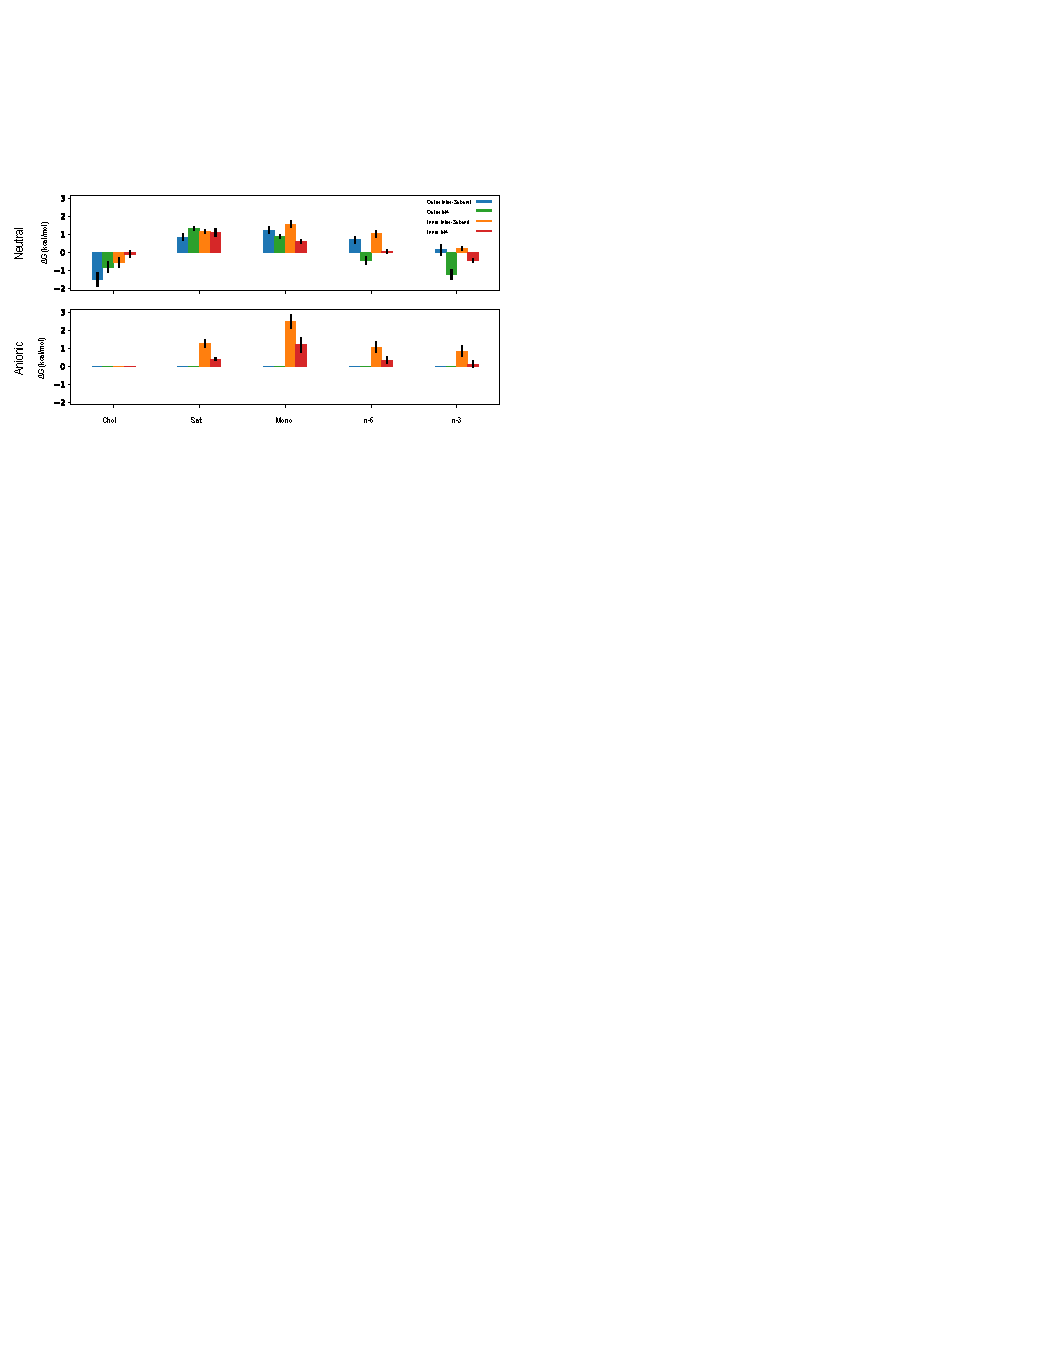
\includegraphics[width=\linewidth]{./Figures/Protein_centric.pdf}
	\caption[\Newaffinities{} organized to reveal site selectivity.] {The \newaffinities ($\Delta G$) are calculated using Equation \ref{eq:dG}, where error bars are the standard error (n=10 independent replicas).  \Newaffinities are colored by site; in the outer leaflet: intersubunit (blue) and  M4 (green), and for the inner leaflet: intersubunit (orange) and M4 (red). Values are separated by headgroup charge (rows) and acyl chain type (columns). More negative values indicate stronger affinities, while more positive values indicate more displacement of the lipid by other lipid species. Data incorporates 10 replicas averaging over the last half of the 5$us$ trajectory, with five-fold averaging over each type of pseudosymmetric site. Figure \ref{fig:lipidBar} has an alternate representation of the same data.  }  % Colors: Outer Inter-Subunit:blue, Outer M4:green, Inner Inter-Subunit:orange, Inner M4:red.}
	\label{fig:proBar}
\end{figure*}

Representative frames from a typical trajectory of boundary lipids are shown in Figure \ref{fig:trj}A, with representative poses shown in Figure \ref{fig:trj}B.  In order to quantitatively compare the lipid distributions for the native system to our previous model system, we plotted the enrichment of boundary density relative to bulk density on a two-dimensional polar heat map centered around the protein. This enrichment is shown in Figure \ref{fig:acyl_map}A for cholesterol and various acyl chains grouped by  saturation. Saturated and monounsaturated acyl chains are not significantly depleted or enriched in the boundary of the protein. Regions of cholesterol density are much more localized than in the model membrane (Figure \ref{fig:acyl_map}C) , with pockets of high enrichment very close to the protein and weak depletion in the remainder of the boundary region.  Both n-6 and n-3 PUFA chains yield five-fold symmetric enrichment around the M4 alpha-helices, as observed for n-3 PUFAs in the model membrane.  In the neuronal membrane, however, this enrichment is less well-defined and spreads into the intersubunit regions. In particular, additional pockets of significant enrichment are apparent in the $\beta-\delta$ subunit interface in the outer leaflet. The overall area of the regions of PUFA-enrichment decrease in the inner leaflet, where n-3 PUFAs are enriched around M4 helices, but n-6 PUFA density is not five-fold symmetric and has weak enrichment. Overall, the loss of definition in site boundaries diverges from the well-defined five fold enrichment for n-3 PUFAs we saw in model membranes\cite{Woods2019}. 

In order to reduce these distributions to affinities that are more straightforward to interpret, we calculated the \newaffinity{}  $\Delta G$ for various lipid species as defined in Eq. \ref{eq:dG}. We organize this information in two different ways: Figure \ref{fig:proBar} provides the ``lipid's perspective'' and is organized to identify the preferred site for a given lipid type (the lipids' ``site selectivity''), while Figure \ref{fig:lipidBar} provides the ``site's perspective'' and is organized to identify the most favorable lipids for a given site (the sites' ``lipid specificity''). 

We first consider site selectivity for neutral lipids. Affinities for neutral lipids and cholesterol are shown in Figure \ref{fig:proBar}A, where more negative values of $\Delta G$ indicate a stronger \newaffinity{} and more positive values indicate more displacement by other lipids.  Overall, as shown in Figure \ref{fig:proBar}A, saturated lipids have similar \newaffinities{} across all sites, which is consistent with the generally flat distribution observed in Figure \ref{fig:acyl_map}. Yet saturated lipids do yield a slightly stronger affinity for intersubunit sites, at least in the outer leaflet, which may drive the high amount of saturated enrichment observed at these sites in model membranes.  Outer leaflet monounsaturated lipids are slightly more unfavorable in intersubunit sites than M4 sites, and this difference grows in the inner leaflet. 

In contrast to saturated and monounsaturated lipids, PUFAs and cholesterol are highly selective for particular sites.  As shown in Figure  \ref{fig:proBar}A, neutral PUFAs have significantly stronger affinities for M4 sites than for innersubunit sites in the same leaflet.  Such selectivity is consistent with the PUFA enrichment density in Figure \ref{fig:acyl_map}A, where n-3 PUFAs can occupy most regions of the TMD but have particularly high levels of enrichment around M4. It is further consistent with our expectations from model membranes (Figure \ref{fig:acyl_map}C). Regardless of the site class, PUFAs favor the outer leaflet site over the inner leaflet site, but both sets of M4 sites are more favorable than both sets of intersubunit sites.  Conversely, cholesterol has significantly stronger affinities for innersubunit sites than for M4 sites, which is also consistent with the enrichment density in Figure \ref{fig:acyl_map}A and our expectations from model membranes (Figure \ref{fig:acyl_map}C). For cholesterol, however, the leaflet is a bigger determinant of affinity than the site; cholesterol has a stronger affinity for either outer leaflet site compared to either inner leaflet site.  

\subsection{Lipid preferences of intersubunit and M4 sites}
We now switch perspectives to considering which neutral lipids are most favorable for particular sites. As shown in Figure \ref{fig:lipidBar} A and B, intersubunit sites in both leaflets prefer cholesterol to phospholipids, which is expected based on the results from model membranes.  Upon visual inspection, this result may appear to diverge from the cholesterol polar density plots in neuronal membranes (Figure \ref{fig:acyl_map} A).  The present results show that while the overall footprint of cholesterol enrichment in (Figure \ref{fig:acyl_map} A) is small, this small region actually reflects a tight and persistently occupied binding site.  The highly right-shifted distributions for cholesterol are shown in Figure S1.  %\grace{LMS: I'm not sure about the following explanation.  Did we discuss this? If so, can we discuss it again? } \liam{we had, though it was my understanding it was roughly the same as what is in the previous sentence.}    We argue difference between weak cholesterol enrichment and strong cholesterol affinity is a result of averaging. For the density analysis, the peak of the the lipid distribution is isolated as a result of averaging, while for the affinity calculation, the full distribution is used to compute the affinity, see Figure SI 1.

PUFA chains yield affinities for the intersubunit site that are approximately $>$0.5 kcal/mol stronger than saturated lipid affinities (Figure \ref{fig:lipidBar} A and B), which was unexpected based on results from model membranes but is consistent with the corresponding enrichment density in Figure \ref{fig:acyl_map}A. More generally, neutral phospholipid affinities for intersubunit sites obey the following trend, from strongest to weakest: n-3 $>$ n-6 $>$ saturated $>$ monounsaturated. Thus, even though PUFA chains prefer M4 sites to intersubunit sites,  and saturated chains prefer intersubunit sites to M4 sites, PUFAs have a stronger affinity for either site type than do saturated lipids. 
 
For intersubunit sites, monounsaturated lipids have the weakest affinities ($>0.5$ kcal/mol), which may reflect a limited number of ways to pack the single kink of a monounsaturated chain in this concave site. In contrast, cholesterol and PUFAs are either small or highly flexible and may more easily pack across multiple sites. Saturated chains may pack parallel to the protein surface in these sites. 
% may pack around inter-subunit site's concave topology. The single acyl-chain kink found in monounsaturated lipids may prevent packing of itself around inter-subunit sites, and is not flexible to compete with PUFA's occupying M4 sites. 

As shown in Figure \ref{fig:lipidBar}C and D, M4 sites in both leaflets have the strongest affinity for n-3 PUFAs, and affinity weakens as acyl chain rigidity increases; from strongest to weakest the phospholipid affinities follow: n-3 $>$ n-6 $>$ monounsaturated $>$ saturated.  This is consistent with a role for PUFAs in minimizing unfavorable membrane deformations caused by the \plgic's conical-star shape.\cite{Brannigan2007,Kim1998,Dan1993,Goulian1996,Goulian1993,Fournier2015}  Surprisingly, cholesterol had a stronger affinity for M4 sites than any acyl chains other than n-3 PUFAs. Cholesterol is rigid, small, and has asymmetric sides (rough and smooth) which potentially allows it to embed between alpha-helices and compete with n-3 PUFAs for binding. Any cholesterol bound within the grooves of the subunit interface (as hypothesized based on atomistic simulations\cite{Brannigan2008} and observed in $\beta$ subunits  of \nachr{} (using coarse-grained simulations\cite{Sharp2019}), will also get counted within the M4 site.   %Cholesterol's favorability for M4 is a result of its size and asymmetric shape, making it ideal for packing between alpha-helices. 

%Unlike phospholipids, cholesterol has the strongest affinity for inter-subunit sites, however cholesterol has affinity values $<0$ kcal/mol at all sites. 
%Figure \ref{fig:lipidBar} shows site affinity for acyl-species, and is sorted by charge and leaflet. Inter-subunit sites in both leaflets has the strongest affinity for cholesterol. 
%M4 sites in both leaflets have the strongest affinity for n-3 PUFAs. Both sites have distinct trends shared across leaflets. Inter-subunit sites have the phospholipid affinity trend: n-3 $<$ n-6 $<$ saturated $<$ monounsaturated, while 
%Cholesterol has the strongest affinity of the neutral lipids at inter-subunit sites for both leaflets, but inner inter-subunit sites affinity is $\sim 50 \%$ weaker. Neutral phospholipids at inter-subunit affinity values change $<0.5$ kcal/mol between leaflets.  Inter-subunit and M4 have different affinities trends: and  respectively. 
 %At the M4 sites, n-3 PUFAs interact more favorably than other lipids 
%\subsubsection{Discussion}
%Of the neutral lipids, n-3 PUFAs and cholesterol stand out. We predict the relative high affinity for n-3 PUFAs are a result of their flexibility. The n-3 PUFA, DHA, has several of unique membrane properties \cite{Stillwell2003a,Gawrisch2003}, and is observed to consistently interact with non-annular sites in and around \plgic s \cite{Sharp2019, Woods2019}. 


\begin{figure*}[!h]
	\center
	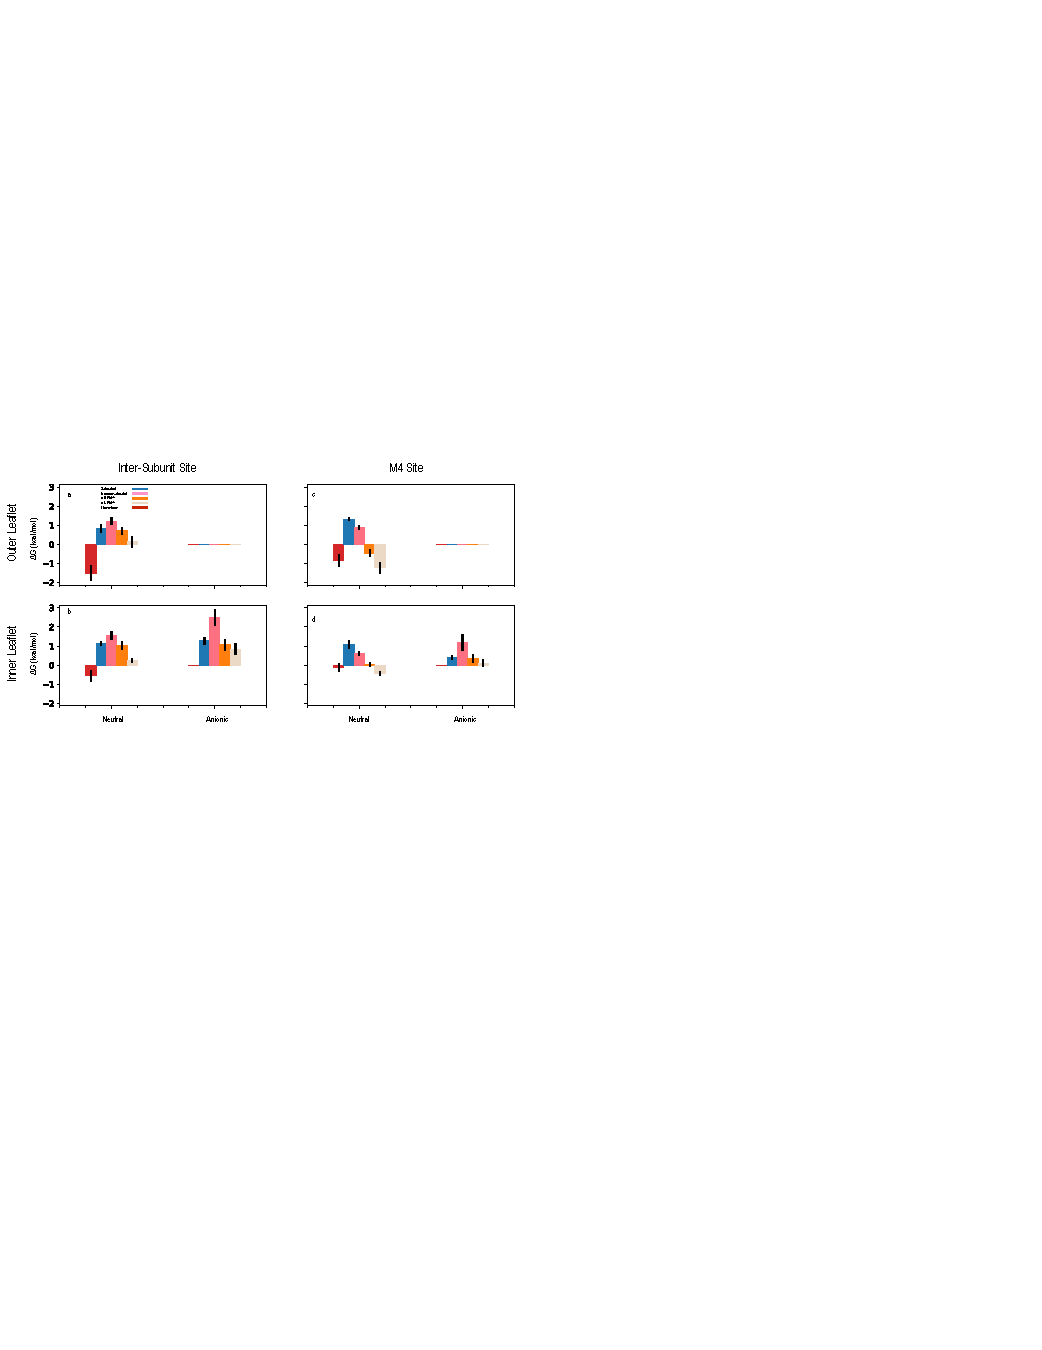
\includegraphics[width=\linewidth]{./Figures/Lipid_centric.pdf}
	\caption[\Newaffinities{} organized to reveal lipid preferences by site.] {Data shown is identical but reorganized and recolored from Figure \ref{fig:proBar}. Here, \newaffinities are colored by chain type (Saturated:blue, Monounsaturated:pink, n-6 PUFAs:orange, n-3 PUFAs:tan, Cholesterol:red), and separated by leaflet (rows) and site (columns).} %More negative values indicate stronger affinities, while more positive values indicate more displacement of the lipid by other lipid species. Data incorporates 10 replicas averaging over the last half of the 5$us$ trajectory, with five-fold averaging over each type of pseudosymmetric site. } {Affinity calculation ranking for neutral and anionic lipid saturation species averaged the final 2.5 $\mu s$ simulations for each 10 replicas by occupancy site. Occupancy sites are averaged from 5 sites.\grace{LMS:Isn't it five sites?} Row one is the outer leaflet and row two is the inner leaflet. Columns are charge, each subplot is a difference occupancy site.  Error bars are the standard error calculated over the 10 replicas simulated. The smaller the number the stronger the affinity. Colors: Saturated:blue, Monounsaturated:green, n-6 PUFAs:orange, n-3 PUFAs:red, Cholesterol:purple}
	\label{fig:lipidBar}
\end{figure*}

\subsection{Effect of Head Group Charge on Affinity Depends on Leaflet and Binding Site}
%Research by Tong et al 2019 \cite{Tong2019} showed anionic lipids favorably occupied around arginines in ELIC's inner inter-subunit site. We hypothesize \nachr's outer TMD and inner inter-subunit sites will have a strong affinity for neutral phospholipids and \nachr's inner M4 sites will have a strong affinity for anionic phospholipids because M4 has more cationic amino acids, see Figure \ref{fig:aaa}a. We test the proposed lipid distributions using both enrichment density analysis and affinity calculations.
Figure \ref{fig:acyl_map}b compares the density enrichment for anionic headgroups with that of neutral headgroups. Data is shown for the inner leaflet only, because anionic lipids are not present in the outer leaflet at the start of simulations and few anionic lipids flip flop to the outer leaflet.% Furthermore, as shown in Figure \ref{fig:lipidBar}C, the anionic lipids that do flip in to the outer leaflet (\grace{LMS: how many is this?}) \liam{I'm not sure. Versions of the manuscript have had comments trying to bring up anionic distributions and affinities with you previously. It looks like 1 - 5 lipids flip? }  have very weak affinity for any sites in the outer leaflet ($\geq 2.0$ kcal/mol). These results are consistent with our previous observations that POPG had very weak affinity for the outer leaflet sites of ELIC\cite{Tong2019}.

In the inner leaflet, the anionic lipids are expected to select for sites that are lined with basic amino acids, which are in different locations depending on subunit (Figure \ref{fig:aaa})  As shown in Figure \ref{fig:acyl_map}b, anionic lipids are generally enriched around the M3/M4 helices for the $\alpha_{\gamma}, \gamma,\delta,$ and $\beta$ subunits.  Anionic lipids are enriched at intersubunit sites and around M4 sites for all subunits but the $\alpha$ subunits. Non-$\alpha$ \nachr~ subunits have basic amino acids closer to M4 alpha-helices, as shown in Figure \ref{fig:aaa}.  We incorporate data from all five pseudo-symmetric sites to obtain the \newaffinities{} reported in Figure \ref{fig:proBar}B, which suggest that anionic lipids have significantly stronger affinities for M4 sites on average. The average anionic affinity difference between inter-subunit and M4 sites is $\sim -1.0$ kcal/mol, as shown in Figures \ref{fig:proBar}, \ref{fig:lipidBar}d and SI \ref{tab:avg_s}. Although the magnitude of the affinity difference varies with acyl chain saturation, the sign is unchanged.     %Neutral lipids have weak enrichment around M4 sites in the outer leaflet, but other wise are neutral.
%We hypothesize the difference in our result is from the number and placement of charged amino acids in ELIC's (TMD PDB:3RQW\cite{Pan2012}) versus that of neuromuscular \nachr. We use VMD \cite{HUMP96} to visualize the difference between \nachr~and ELIC's inner \notsure{leaflet} TMD, . Both pLGICs have a number of cationic amino acids around their annulus. ELIC has more cationic amino acids embedded in the protein density than at the annulus. \notsure{Cationic amino acids found in the \nachr~structure tend to be more outward facing than cationic amino acids in the ELIC structure.} Non-$\alpha$ \nachr~ subunits have cationic amino acids closer to M4 alpha-helices. ELIC has cationic amino acids closer to the inter-subunit sites. Anionic amino acids are found at \nachr M4 alpha-helices, with the exception of the $\beta$ subunit. Anionic amino acids are found closer to the M1/M4 alpha-helices interfaces in ELIC, or embedded within the \liam{inner/non-annular/bulk of} protein.
%At inter-subunit sites the same trend with acyl-chain persists: n-3 PUFAs $>$ n-6 PUFAs $>$ saturated $>$ monounsaturated.  %In the outer leaflet, \nachr~ has preferential binding with cholesterol, neutral PUFAs, and then monounsaturated or saturated, the later are dependent on site.  
We now switch again to the ``site perspective'' to compare whether inner leaflet sites would prefer occupancy by anionic or neutral lipids. % compare the affinity of anionic lipids for inter-subunit sites the lower leaflet, see Figure \ref{fig:lipidBar}b. 
As shown in Figure \ref{fig:lipidBar}C, lipid affinity values for inter-subunit sites are either insensitive to charge (saturated or n-6 PUFA chains) or weaker for anionic lipids by at least 0.5 kcal/mol (monounsaturated and n-3 PUFA chains).  In comparison, at the M4 site, saturated chains in anionic lipids have significantly stronger affinities than those in neutral lipids (a difference of $\sim$0.5 kcal/mol). All other lipid chains attached to anionic headgroups have weaker affinities for the M4 site. The clear trend observed in neutral lipids (stronger affinities for more flexible acyl chains) is thus broken in anionic lipids because saturated anionic lipids are so favorable.  %Anionic lipids in the inner leaflet have affinities $\sim 1.0$ kcal/mol stronger than in the outer leaflet, monounsaturated lipids are an exception.
% Anionic affinities are more favorable at inner inter-subunit sites than the outer leaflet, difference $\sim1.0$ kca/mol, excluding monounsaturated lipids. % have $\sim 1.0$ kcal/mol stronger affinity for the inter-subunit sites than in the outer leaflet.

%Next we compare the relative affinities for anionic lipids occupying M4 sites in the lower leaflet, see Figure \ref{fig:lipidBar}d. Unlike the inter-subunit sites,  anionic and neutral lipids have different affinity trends:  Anionic lipids continue to be non-monotonic: n-3 PUFAs $>$ n-6 PUFAs $>$ saturated $>$ monounsaturated, where neutral lipid affinities are related to the acyl-chain flexibility, the stronger the affinity the more flexible the acyl-chain. Anionic lipids are generally $<0.6$ kcal/mol, excluding monounsaturated lipids. Anionic lipids have stronger occupancy affinity values at M4 than at inter-subunit sites, regardless of saturation. 
%\subsubsection{Discussion}
In summary, we observe that binding sites have clear preferences for particular head group charge and acyl-chain saturation, suggesting \nachr~lipid occupancy to be driven in two steps, a ``coarse-sorting'' by head groups, and then ``fine-sorting'' by acyl-chains.  A neutral lipid will occupy \nachr's boundary region but acyl chains dictate where specific lipids occupy \nachr. Anionic lipids diverge from this pattern at the inner M4 site which has the strongest affinity for anionic lipids independent of saturation. 
%A potential mechanism for anionic lipid site occupation could be anionic lipids occupy M4 due to the number of positively charged amino acids until the site is saturated with anionic lipids, similar to Tong et al\cite{Tong2019}. The remainder anionic lipids do not all defuse back to the bulk membrane, they weakly interact with the inner inter-subunit site as a local anionic lipid pool for M4. 
\subsection{Role of Individual Lipid Headgroups in Determining Affinity}
%The NEW SECTION 3.3 : EFFECT OF HEADGROUP DETAILS ON LIPID AFFINITIES can instead be focused on the effect of specific headgroups
%Neutral lipids have a higher affinity in the outer leaflet. Neutral and anionic lipids show a level of competition at inner inter-subunit sites.  Anionic lipids have an acutely stronger affinity at inner M4 sites compared to neutral lipids. 
Neutral and anionic are bulk terms that categorize numerous lipid head-groups by charge. %Frequently head group charge and size play a factor in direct protein-lipid interactions. 
To understand the role of the chemical distinctions between head groups of like charge, we broke the headgroup affinities down by headgroup species in Table \ref{tab:dGOuterHG}.  %we introduce the anionic lipids with the strongest affinities for occupying \nachr~by leaflet and site.
%We measure head group affinities in the outer leaflet site, see Table \ref{tab:dGOuterHG}.  
In the outer leaflet, lipids contain a mixture of PE and PC headgroups. The small neutral PE head group has the strongest affinity across all headgroups for both inter-subunit and M4 sites, -0.2$\pm$0.3 and -1.1$\pm$0.2 kcal/mol respectively. The larger neutral PC headgroups are weaker than PE by $\sim > 0.5$ kcal/mol. In living cells, as in this neuronal membrane, PUFAs are more frequently tethered to PE than to PC or SM \cite{Isolated1969, Taguchi2010, Breckenridge1973,Ingolfsson2017b,Lorent2020}, so it is possible that this affinity simply reflects the high affinity of PUFA chains. However, even for identical chains, both experimental and simulation data \cite{Sharp2019} suggests stronger PE-ELIC than PC-ELIC interactions.  

Table \ref{tab:dGInnerHG} shows specific head group affinities in the inner leaflet. %Anionic lipids have a stronger  affinity in the inner leaflet compared to the outer leaflet, especially at the M4 sites. 
As in the outer leaflet, lipids with PE headgroups still have the strongest affinity of all lipids, but in the inner leaflet we are also able to distinguish affinities for anionic species. For the intersubunit site, PI, PS, and PC have similar affinities (within statistical error), and have significantly stronger affinities for these sites than the phosphoinositides (PIPS) PIP1, PIP2, PIP3, which have a significantly stronger affinity than phosphatidic acid  (PA). Thus, from strongest to weakest, PE$>$PI$\sim$PS$\sim$PC$>>$PIP1$\sim$PIP2$\sim$PIP3$>>$PA for the intersubunit site. In contrast, at the M4 site, more significant differences among moderate affinity headgroups emerge. PI has significantly stronger affinity than PS (a difference of 0.3$\pm$0.1 kcal/mol), and PS has a significantly stronger affinity than PC (a difference of 0.2$\pm$0.1 kcal/mol).% \grace{LMS please fill in the missing values. You may have them in some text I commented out, but I couldn't be sure. To get an overall error difference, remember that the error in X1 - X2 is $\sqrt{dx1^{2} + dx2^{2}}$ where dx1 and dx2 are the individual errors.} \liam{$\sqrt{dx1^{2} + dx2^{2}}$ is .14 for both PI vs PS and PS vs PC, rounded to .1}
From strongest to weakest, PE$>$PI$>$PS$>$PC$>>$PIP1\\$\sim$PIP2$\sim$PIP3$\sim$PA for the M4 site.    %PI and PS are $\sim 0.4 $ and $\sim 0.6$ kcal/mol weaker than PE (inter-subunit and M4 respectively), they are $\sim 0.1$ and $\sim0.4$kcal/mol stronger than PC at inter-subunit and M4 sites respectively. Other anionic lipids, phosphatidic acid  (PA) and phosphoinositides (PIPS) have affinity values $>2.2$ and $>1.8$ kcal/mol for inter-subunit and M4 sites respectively. 

%Sharp et al 2019\cite{Sharp2019} and Tong et al 2019\cite{Tong2019} observed slightly more enrichment of PE than PC around pLGICs. 

%\subsubsection{Discussion}

\begin{table}
	\caption[\Newaffinities () of neutral lipids for both sites in the outer leaflet, by head group.]{  Errors are standard errors (n=10 independent replicas). }
    \centering
    \begin{tabular}{|l||c|c|}
    \hline
	{} &   Intersubunit Sites&  M4 Sites\\
	{} & $\Delta$G (kcal/mol) & $\Delta$G (kcal/mol)\\
	\hline
	PE	&-0.2 $\pm$ 0.3& -1.1$\pm$0.2\\
	%PC	& 0.8 $\pm$0.3 &  0.5$\pm$0.2\\
	PC & 1.4$\pm$0.2&	1.1 $\pm$0.2\\
	%SM	&1.9$\pm$0.3 &  1.7$\pm$0.1\\
	\hline
    \end{tabular}
    \label{tab:dGOuterHG}
\end{table}

\begin{table}
	\caption[\Newaffinities ($\Delta$G) of neutral lipids for both sites in the inner leaflet, by head group.] {Values are sorted by strength of affinity for intersubunit sites. Errors are standard errors (n=10 independent replicas). }
    \centering
    \begin{tabular}{|l||c|c|}
    \hline
	{} &  Inner Inter Sites&  Inner M4 Sites\\
	{} & $\Delta$G (kcal/mol) & $\Delta$G (kcal/mol) \\
	\hline
	PE& 0.3$\pm$0.2& -0.1$\pm$0.1\\
	PI&0.9$\pm$0.3 &  0.2$\pm$0.1\\
	PS&1.0 $\pm$0.2	&  0.4$\pm$0.1\\
	%PC&1.2 $\pm$0.2	&  0.7$\pm$0.1\\\
	PC &1.0$\pm$0.2 &	0.9$\pm0.1$ \\
	%SM&2.2 $\pm$0.4	&  1.4 $\pm$0.1\\
	PIP3	&2.6$\pm$0.4	 &  1.8 $\pm$0.4\\
	PIP2	&2.8 $\pm$0.2	&  2.1$\pm$0.4\\
	PIP1	&2.4 $\pm$0.3	&  2.1$\pm$0.4\\
	PA	&3.0 $\pm$0.3	&  2.2$\pm$0.4\\
	\hline
    \end{tabular}
    \label{tab:dGInnerHG}
\end{table}

\section{Conclusions}

\label{con}

Using coarse-grained simulations of the \nachr{} within a quasi-neuronal membrane containing over thirty lipid species, we have observed spontaneous lipid binding and quantified lipid specificity for two types of sites in the protein TMD.  These two site classes represent the most concave (intersubunit site) and convex (M4 site) portions of the star-shaped \nachr~ and were initially observed as ``hot spots'' in our previous simulations\cite{Woods2019,Tong2019} of model membranes. Compared to classic ligand binding sites, these sites are superficial and have a large volume. The ``ligands'' occupying them are also non-traditional: lipids are flexible chain molecules that may only partially occupy the site and are likely to share the site with other partially-occupying ligands.  While our lab has developed promising alchemical approaches\cite{Salari2018} for calculating traditional affinities of atomistic lipids for more highly localized, well-defined sites, these hot spots required a different approach. Here we have proposed a softer ``\newaffinity'' for characterizing these affinities from spontaneous, unbiased coarse-grained simulations. While we restrict the use of this method here to \nachr, it should be straighforward to extend to any other transmembrane proteins with detectable regions of density enrichment. 

\begin{figure}
	\center
	%\includegraphics[width=\linewidth]{Summary.pdf}
	\includegraphics[width=3.5in]{./Figures/Summary.pdf}
	\caption[Cartoon of expected boundary lipids for the \nachr~ in a native membrane for both leaflets.] {Protein is shown in the center of both leaflets in a cyan floral shape. Grey and black outlines depict sites favorable for neutral and anionic lipids respectively. Fill color represents the lipids most likely to occupy each site (red: cholesterol, blue: saturated, beige: PUFA) and outline represents headgroup charge (gray: neutral, black: anionic).}
	\label{fig:sum}
\end{figure}

Our results are summarized graphically in Figure \ref{fig:sum}. Based on our results from model membranes, we had hypothesized that
%We used a neuronal lipid compositions modified from\cite{Ingolfsson2017b} to analyze \nachr~within a neuronal membrane. We defined lipid-protein occupancy from polar enrichemnt density plots and used Sharp\cite{Sharp2019}, Woods\cite{Woods2019}, and Tong\cite{Tong2019} to hypothesized lipid occupancy for each site. We hypothesized 
 PUFAs would select for the convex M4 sites and that raft-forming lipids like cholesterol and saturated lipids would select for the concave inter-subunit sites. Overall, our results were consistent with this expectation.  Yet although lipids containing PUFAs do prefer the M4 site to the intersubunit site, their affinity for even the intersubunit sites are stronger than that of all other phospholipids. This result underscores the reliable partitioning of \nachr{} to PUFA-rich, liquid-disordered domains that we observed in homoacidic, domain forming membranes\cite{Sharp2019}, and suggests PUFAs may have been absent from the intersubunit site in heteroacidic membranes\cite{Woods2019} because of the constraints of the lipid topology. In the latter simulations, all lipids contained one saturated chain and one PUFA chain, so binding of the PUFA chain to its preferred M4 site requires the saturated chain to find the most favorable location nearby (in the intersubunit site) and may block binding of other PUFA chains to that site.  These constraints are relaxed in the native neuronal membrane, which has a more diverse lipid composition with multiple different chain pairings; about 6\% of the phospholipids in our simulated membranes contain no saturated chain at all. Nonetheless, our previous results\cite{Woods2019} using simplified binary heteroacidic/cholesterol membranes played a key role in identifying the natural site boundaries.  

As expected, within each leaflet cholesterol has the strongest affinity for the inter-subunit sites, although the affinity of cholesterol for the M4 sites was second only to that of n-3 PUFAs. Combined, these results are consistent with an overwhelming amount of evidence spanning four decades that suggests direct interactions between cholesterol and \nachr s, regardless of the phospholipid composition of the membrane.  One surprise for cholesterol was the role of the leaflet in determining affinity: cholesterol has a stronger affinity for either outer leaflet site compared to either inner leaflet site. This result may reflect competition with anionic saturated lipids in the inner leaflet, which would be consistent with multiple experiments\cite{Baenziger2000,Wenz2005,Hamouda2006,Thompson2020}, suggesting that anionic lipids can partially or fully compensate for a loss of cholesterol.  This result is also consistent with cholesterol embedded\cite{Brannigan2008} in the outer TMD (which has numerous gaps in the amino acid density) but not the inner TMD. 
%Of the phospholipids analyzed, n-3 PUFAs have the strongest affinities across all sites, with affinities values of $\sim<0$ kcal/mol for M4 sites and $\sim<$.5 kcal/mol for inter-subunit sites. %We predict the relative high affinity for n-3 PUFAs are a result of their flexibility. The n-3 PUFA, DHA, has a number of unique membrane properties \cite{Stillwell2003a,Gawrisch2003}, and is observed to consistently interact with non-annular sites in and around \plgic s \cite{Sharp2019, Woods2019}. The inherent disorder in PUFAs and the strong affinity they have for M4 sites suggests PUFAs may minimize unfavorable membrane deformation\cite{Brannigan2006,Brannigan2007,Hu2012a,Argudo2016a,BuganzaTepole2017,Dan1993,Fournier2015} around \plgic's conical-star shape provided by M4.
%Similar to n-3 PUFAs cholesterol occupies sites nearly indiscriminately, though for each leaflet cholesterol has the strongest affinity at inter-subunit site. Cholesterol's affinity for the M4, compared to inter-subunit sites, is reduced by about $50\%$ and $80\%$ for the outer and inner leaflets respectively. However, unlike the phospholipids, cholesterol's affinity for each site is consistently $<0$ kcal/mol. %Brannigan et al 2008 \cite{Brannigan2008} hypothesized 15 non-annular cholesterol binding sites for \nachr. Sharp et al 2019 \cite{Sharp2019} observed cholesterol embedded in $\beta$ subunits of \nachr. It could be cholesterol's favorability for M4 is a result of its relative small size making it ideal for packing between alpha-helices.

%For most sites monounsaturated lipids have the weakest affinities ($>.5$ kcal/mol). We hypothesize this is due to packing limitation from monounsaturated lipids single acyl-chain kink. Cholesterol and PUFAs are small or highly flexible and readily fit at various sites in \plgic's topology. Saturated lipids, which lack any kinks and are more rigid than unsaturated lipids, may pack around inter-subunit site's ''flat'' topology. We argue the single acyl-chain kink found in monounsaturated lipids may prevent packing of itself around inter-subunit sites, and is not flexibility to compete with PUFA's occupying M4 sites. 

%Neutral lipids that occupy M4 have a unique trend in affinity. The affinity strength increase as a relation to acyl-chain flexibility, initially state in section \textit{Effect of Acyl-Chain on Neutral Lipid Affinities}. Neutral lipids at inter-subunit sites and all anionic lipids share a non-monotonic affinity trend where it is more akin to a concave function, see Figure \ref{fig:sum}. 

Based on our results using ELIC\cite{Tong2019}, we had expected that anionic lipids would select for sites on the inner leaflet lined with basic residues.  In the homomeric ELIC, these residues are symmetricly-arranged, while in the heteromeric \nachr{} they vary by subunit(Figure \ref{fig:aaa}a), with the M4 site containing the most such residues on most subunits. The present results support that expectation: %Yet unlike ELIC due to cationic amino acid distribution, see Figure \ref{fig:aaa}a. \nachr~ has cationic amino acids at both inter-subunit and M4 sites.
%Neutral lipids have a stronger affinity for the outer leaflet compared to anionic lipids. Neutral lipids found at the inner inter-subunit sites have slightly weaker affinities compared to the same lipids in the outer inter-subunit site. 
anionic lipids have a stronger affinity for M4 than inter-subunit sites.  %Inner anionic saturated, n-6 and n-3 PUFAs have significantly greater affinities than outer anionic lipids of the same saturation types. Monounsaturated lipids affinity values do not change much between leaflets ($\sim 0.5$ kcal/mol). We associate anionic lipids have stronger affinity for M4 in \nachr~compared to ELIC due to cationic amino acid distribution, see Figure \ref{fig:aaa}a. \nachr~ has cationic amino acids at both inter-subunit and M4 sites.

For both outer and inner leaflets, neutral lipids with smaller head groups (PE) have stronger affinity than the larger PC headgroup. It is unclear why PE is more favorable than other neutral lipids at this time, though this is consistent with previous work \cite{Sharp2019,Tong2019}, and the most straightforward explanation is that the smaller headgroup introduces fewer clashes with the protein TMD. % It may be due to the frequency which PE are attached to lipids with PUFAs or the size of the head group.  However, many of the the anionic lipid head groups are attached to PUFAs.

Among anionic lipids in the inner leaflet, regardless of the site, PS and PI have an affinity greater than or equal to PC, and much greater than the other anionic lipid headgroups (PIP1,PIP2,PIP3, and PA).   The lipid headgroups PS and PI both have a charge of -1, while PA in the MARTINI forcefield\cite{DeJong2012} carries a charge of -2, and PIP1, PIP2, and PIP3 have charges of -3,-5, and -7. These results suggest that the inner leaflet sites select for monoanionic headgroups, while multianionic headgroups are highly unfavorable.  Due to the limitations of the coarse-grained model, future atomistic calculations are required to validate and understand the apparent preference of the M4 site for PI over PS.  %These differences cannot be attributed to size alone: the bulkier PI (four martini beads) and the small PS (two martini beads) have comparable affinities which are both much greater than both the bulky PIPS and the smallest headgroup, PA. 

The present results highlight the utility of model membranes for developing hypotheses of specific lipid-protein interactions, and the need to test those hypothesis within more complex native membranes. The present results could be tested and aid in interpretation of experiments carried out in more complex membranes. For instance, we would expect that mutations of the basic residues facing the inner leaflet would reduce binding of saturated phospholipids with anionic headgroups, which would be replaced with bound cholesterol. We would also predict that if PUFAs cause gain of function via binding to the intersubunit site, this gain would be enhanced by replacing some heteroacidic lipids with homoacidic lipids while keeping the total fraction of PUFA chains constant. In general the present results provide valuable insight into how to predict lipid competition, which is one of the primarily challenges of interpreting experiments in complex membranes.  
%.  PA has the weakest affinity of the anionic lipids, though it has the smallest head group (only a phosphate), and PIPS which are much bulkier than all the other head groups are comparable to PA. PI, PS  share the same charge: -1.0 C. 


%Why one head group interacts more favorably is still unknown. It may be a product of head group to acyl-chain combination, evolution, or the coarse grained model. The PE head group bead types are Qd and Qa, which are attracted to most of the other bead types. PS has P5 and a QA, where P5 is attractive to about half the bead types and repulsive to the other half. PI has coarse-grained ring of P5 and P1s, and Qa, all of which tend to be attractive to other beads.  



%It is unclear why neutral and anionic head group affinities are uncorrelated, though it may be a product of head group to acyl-chain combination, evolution, or the coarse grained model. \notsure{The PE head group bead types are Qd and Qa, which are attracted to most of the other bead types. PS has P5 which is attractive to about half the bead types and repulsive to the other half. PI has coarse-grained ring of P5 and P1s, and Qa, all of which tend to be attractive to other beads. }

%\nachr~lipid occupancy appears to be driven in two steps. First a ''coarse-sorting'' by head groups, and second ''fine-sorting'' by acyl-chains. In the outer leaflet anionic lipids are clearly unfavorable, coarse-sorting. A neutral lipid will occupy \nachr's boundary region and then there is ''fine-sorting'' by acyl-chain saturation. Inner Inter subunit sites have competition between lipid head group charge, but have specific acyl-chain affinity. The inner M4 site has the strongest affinity for anionic lipids regardless of saturation type, which diverges from the proposed occupancy driver. 
%
%Inner anionic lipid occupancy could be driven by another mechanism: anionic lipids occupy M4 due to the number of positively charged amino acids until the site is saturated with anionic lipids, similar to Tong et al\cite{Tong2019}. The remainder anionic lipids do not defusing back to the bulk membrane, they weakly interact with the inner inter-subunit site as a local anionic lipid pool for M4. 

% Raft forming lipids have higher affinities for inter-subunit sites over M4, but cholesterol has unexpectedly strong affinity for all sites. Unsaturated lipids have a highest affinity for M4, however, n-3 PUFAs show strong affinity for inter-subunit sites as well  with a difference of about 1 kcal/mol. These results suggest when neutral lipids are available for \nachr's boundary membrane, degree of saturation and molecule size play vital roles. Saturated and monounsaturated lipids, which tend to maintain a higher degree of order when compared to  PUFAs, show poor affinity in-comparison to more flexible lipids. While, saturated and monounsaturated lipids show relative high and low affinity sites within their saturation species, highly flexible PUFAs and small cholesterol occupy \nachr's density gaps more readily.


\section*{Acknowledgments}
GB and LS were supported by the Busch Biomedical Foundation. This project was supported by generous allocation through the Rutgers University Office of Advanced Research Computing (OARC), which is supported by Rutgers University and the state of New Jersey. We are grateful to Dr. J{\'{e}}r{\^{o}}me H{\'{e}}nin for helpful input and suggestions.

\section*{Data Availability Statement}
The data that support the findings of this study are available from the corresponding author upon reasonable request. Scripts for polar density analysis and plotting scripts can be found on github: https://github.com/BranniganLab/densitymap. 
%Using $\Delta G$ free energy to calculate the occupancy affinities, we find n-3 PUFAs and cholesterol \textit{nearly} indiscriminately occupy any region of the protein, cholesterol favors inter-subunit sites and n-3 PUFAs favor M4 sites. Anionic lipids are unfavorable in the outer leaflet. Anionic lipids and neutral lipids occupy at comparable affinities in the inner inter-subunit sites, see Figure \ref{fig:sum}.

%These results show a significant divergence from our proposed hypothesis and are depicted in figure \ref{fig:sum}. In the outer leaflet neutral have a strong affinity to occupy sites. Unsaturated lipids and cholesterol occupy the M4 site, while n-3 PUFAs, cholesterol, and saturated lipids occupy inter-subunit sites. Neutral and anionic lipids occupy inner inter-subunit sites with similar lipid composition compared to the outer leaflet. Inner M4 sites have a strong affinity for anionic lipids regardless of acyl chain.

%% The Appendices part is started with the command \appendix;
%% appendix sections are then done as normal sections
%% \appendix

%% \section{}
%% \label{}

%% References
%%
%% Following citation commands can be used in the body text:
%% Usage of \cite is as follows:
%%   \cite{key}          ==>>  [#]
%%   \cite[chap. 2]{key} ==>>  [#, chap. 2]
%%   \citet{key}         ==>>  Author [#]

%% References with bibTeX database:

%\bibliographystyle{model1-num-names}
%\bibliography{Paper_Bibs}

%% Authors are advised to submit their bibtex database files. They are
%% requested to list a bibtex style file in the manuscript if they do
%% not want to use model1-num-names.bst.

%% References without bibTeX database:

% \begin{thebibliography}{00}

%% \bibitem must have the following form:
%%   \bibitem{key}...
%%

% \bibitem{}

% \end{thebibliography}
%\begin{table}
%    \caption{Lipid ratios used for neuronal simulations grouped by head group.}
%    \label{tab:rats}
%    \centering
%
%\begin{tabular}{|c||c|cc|}
%
%\hline
%Head Group & Lipids & Outer (\%) &{Inner (\%)} \\ \hline\hline
%{}&CHOL                         & 44.3     & 40.67                         \\
%\hline
%PC &{} &30.5&15\\ \hline
%{} &DPPC                         & 6.7      & 3.3                           \\
%{} &DOPC                         & 2.8      & 1.4                           \\
%{} &POPC                         & 11     & 5.4                         \\
%{} &PFPC                         & 0.7      & 0.4                           \\
%{} &PAPC                         & 5.9      & 2.9                           \\
%{} &PUPC                         & 2.1      & 1.0                           \\
%{} &OIPC                         & 0.7      & 0.4                           \\
%{} &OUPC                         & 0.5      & 0.3                           \\
%\hline
%\hline
%PE &{} &13.8&23.4\\ \hline
%{} &POPE                         & 1.6      & 2.7                           \\
%{} &PAPE                         & 4      & 6.7                           \\
%{} &PUPE                         & 6.3      & 10.7                          \\
%{} &OIPE                         & 0.2      & 0.3                           \\
%{} &OAPE                         & 0.9      & 1.5                           \\
%{} &OUPE                         & 0.9      & 1.5                          \\
%\hline
%\hline
%SM &{} &11.3&2.5\\ \hline
%{} &DPSM                         & 7.4      & 1.7                           \\
%{} &PBSM                         & 1.4      & 0.3                           \\
%{} &POSM                         & 0.9      & 0.2                           \\
%{} &PNSM                         & 1.7     & 0.4                           \\
%\hline
%\hline
%PS &{} &0.0&10.8\\ \hline
%{} &DPPS                         & 0.0      & 0.5                           \\
%{} &POPS                         & 0.0      & 2.7                           \\
%{} &PAPS                         & 0.0      & 3.0                           \\
%{} &PUPS                         & 0.0      & 3.8   			\\      
%{} &OUPS                         & 0.0      & 0.8                           \\
%\hline       
%\hline          
%PA &{} &0.0&0.4\\ \hline
%{} &POPA                         & 0.0      & 0.1                          \\
%{} &PAPA                         & 0.0      & 0.3                           \\
%\hline
%\hline
%PI &{} &0.0&2.3\\ \hline
%{} &POPI                         & 0.0      & 1.4                         \\
%{} &PIPI                         & 0.0      & 0.6                           \\
%{} &PAPI                         & 0.0      & 1.4                           \\
%{} &PUPI                         & 0.0      & 2.3                           \\
%\hline
%\hline
%PIPS &{} &0.0&1.5\\ \hline
%{} &POP1                         & 0.0      & 0.2                           \\
%{} &PAP1                         & 0.0      & 0.3                           \\
%{} &POP2                         & 0.0      & 0.2                           \\
%{} &PAP2                         & 0.0      & 0.3                           \\
%{} &POP3                         & 0.0      & 0.2                           \\
%{} &PAP3                         & 0.0      & 0.3                           \\
%\hline
%\end{tabular}
%\end{table}
%
%\begin{figure*}[!h]
%	\center
%	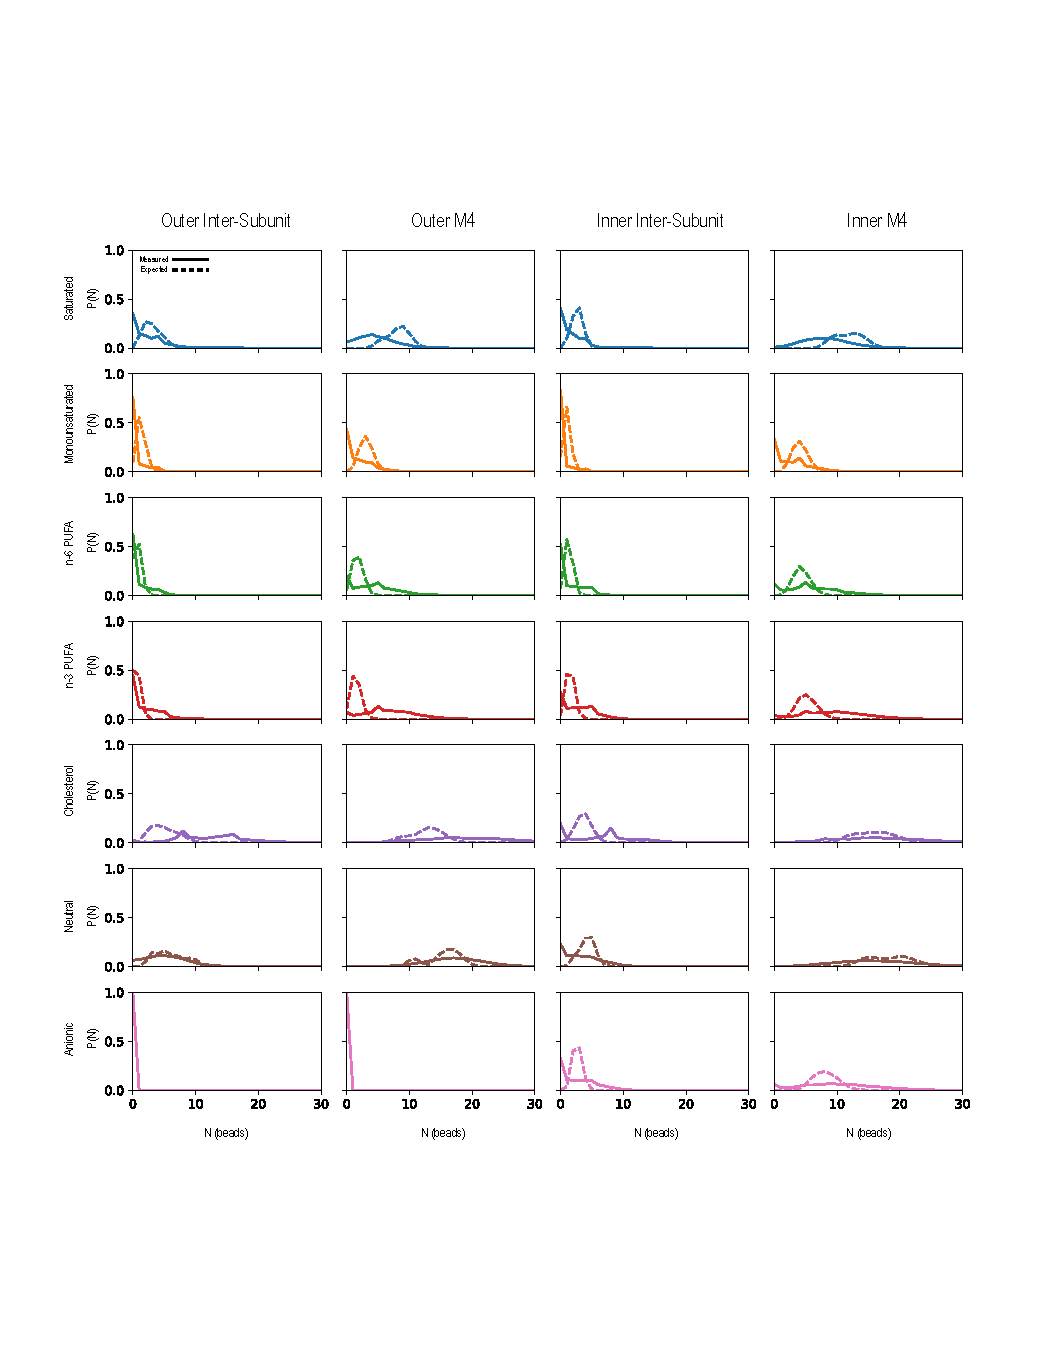
\includegraphics[width=\linewidth]{Bead_Distributions.pdf}
%	\caption{SI:Probability distributions of acyl-chain saturations, including cholesterol, and head group charge. Solid lines are probability of a given number of beads found at occupancy site, averaged over both the course of the simulation and subunit sites. Dashed lines represent the probability of a given number of beads in the bulk averaged over time. Bulk areas are square areas of equal area of occupancy sites.}
%	\label{fig:lipidDist}
%\end{figure*}
%
%\begin{table*}
%    \caption{Affinity values averaged over 10 replicas. $\Delta G$ values for averaged occupancy sites.}
%    \centering
%  \resizebox{\textwidth}{!}{  \begin{tabular}{|l||cc|cc|}
%        
%        \hline
%        {} &  Outer Inter Sites&  Outer M4 Sites&  Inner Inter Sites&  Inner M4 Sites\\
%        {} & kcal/mol & kcal/mol & kcal/mol & kcal/mol \\
%        \hline
%        
%        CHOL &-1.5 $\pm$0.4& -0.8$\pm$0.3&    -0.6$\pm$0.3& -0.1$\pm$0.2\\
%        Sat   &  0.7 $\pm$0.3	&  1.3 $\pm$0.2&     1.0 $\pm$	0.2&  1.1 $\pm$0.2 \\
%        Mono   &    1.2 $\pm$0.2&  0.8$\pm$	0.2&     1.4 $\pm$0.1&  0.7 $\pm$0.2\\
%        n-6   &         0.6 $\pm$0.2& -0.5 $\pm$0.1&0.3 $\pm$0.2& -0.3 $\pm$0.2\\
%        n-3   &       -0.0 $\pm$0.4& -1.3 $\pm$0.3&    -0.2$0.2\pm$ & -0.9$\pm$0.2\\
%        \hline
%        Neutral &     0.4 $\pm$0.3& -0.4$\pm$0.2 &     0.5 $\pm$0.2&  0.5$\pm$0.2 \\
%        Anionic &     2.4 $\pm$0.4&  2.4 $\pm$0.4&     0.3 $\pm$0.2& -0.3 $\pm$0.1\\
%	\hline
%        \hline
%        Sat Neutral &  0.8 $\pm$0.2&  1.3 $\pm$0.1&     1.1$\pm$0.1 &  1.1 $\pm$0.2\\
%        Mono Neutral & 1.2$\pm$0.2&  0.9 $\pm$0.1&     1.6 $\pm$0.2&  0.6 $\pm$0.1\\
%        n-6 Neutral &  0.7 $\pm$0.2& -0.5 $\pm$0.2&     1.0 $\pm$0.2&  0.0 $\pm$0.1\\
%        n-3 Neutral &  0.1 $\pm$0.3& -1.2$\pm$0.3& 0.2 $\pm$0.1& -0.4 $\pm$0.1\\
%        \hline
%        \hline
%        Sat Anionic & 2.5 $\pm$0.4&2.4$\pm$0.4& 1.3$\pm$0.2 &  0.4$\pm$0.1\\
%        Mono Anionic &3.0$\pm$0.5&2.7 $\pm$0.5& 2.5 $\pm$0.4&  1.2 $\pm$0.4\\
%        n-6 Anionic &2.9 $\pm$0.5	&2.7 $\pm$0.5&1.1 $\pm$0.3&  0.3$\pm$0.2\\
%        n-3 Anionic &2.8 $\pm$0.5	& 2.6 $\pm$0.5	& 0.8 $\pm$0.3&  0.1 $\pm$0.2\\
%        \hline
%
%        \hline
%        
%    \end{tabular}}
%    \label{tab:dGTab}
%\end{table*}
%
%\begin{table}
%    \caption{Affinity values averaged over 10 replicas. $\Delta G$ values for each occupancy sites.}
%    \centering
%\resizebox{\textwidth}{!}{\begin{tabular}{| c || cccccccccccccccccccc |}
%\hline
%   Lipids     & Outer $\alpha_{\gamma}-\beta$  & Outer $\beta-\delta$ & Outer $\delta-\alpha_{\delta}$  & Outer $\alpha_{\delta}-\gamma$  & Outer \gamma-\alpha_{\gamma}$  & Outer $\alpha_{\gamma}$   & Outer $\beta$   & Outer $\delta$    & Outer $\alpha_{\delta}$   & Outer $\gamma$   & Inner $\alpha_{\gamma}-\beta$  & Inner $\beta-\delta$  & Inne$\delta-\alpha_{\delta}$ & Inner $\alpha_{\delta}-\gamma$  & Inner $\gamma-\alpha_{\gamma}$  & Inner $\alpha_{\gamma}$    & Inner$\beta$   & Inner $\delta$    & Inner $\alpha_{\delta}$    & Inner $\gamma$   \\
%        \hline
%        & (kcal/mol) & (kcal/mol) & (kcal/mol) & (kcal/mol) & (kcal/mol) & (kcal/mol) & (kcal/mol) & (kcal/mol) & (kcal/mol) & (kcal/mol) & (kcal/mol) & (kcal/mol) & (kcal/mol) & (kcal/mol) & (kcal/mol) & (kcal/mol) & (kcal/mol) & (kcal/mol) & (kcal/mol) & (kcal/mol) \\ \hline \hline
%Lipid Species &&&&&&&&&&&&&&&&&&&&\\\hline
%CHOL    & -0.9       & -1.4       & -1.5       & -1.6       & -2.0       & -1.0       & -1.3       & -0.8       & -0.8       & -0.2       & -0.4       & -0.4       & -1.1       & 0.3        & -1.2       & -0.3       & 0.2        & -0.4       & -0.3       & 0.3        \\
%DOPC    & 3.5        & 3.4        & 2.2        & 2.8        & 2.3        & 1.8        & 2.1        & 1.5        & 1.5        & 1.9        & 2.4        & 3.1        & 2.9        & 2.6        & 2.9        & 1.6        & 1.4        & 1.8        & 1.5        & 1.6        \\
%DPPC    & 3.3        & 2.1        & 2.3        & 1.4        & 2.0        & 1.3        & 2.0        & 1.7        & 2.2        & 1.8        & 1.9        & 2.7        & 2.1        & 2.3        & 2.1        & 1.1        & 1.1        & 1.4        & 1.2        & 1.3        \\
%DPPS    & 4.1        & 4.1        & 4.2        & 3.9        & 4.2        & 3.5        & 3.8        & 3.7        & 3.7        & 3.6        & 4.4        & 4.2        & 3.5        & 4.9        & 5.3        & 2.2        & 2.6        & 2.9        & 2.6        & 3.1        \\
%DPSM    & 2.1        & 2.7        & 2.3        & 1.2        & 2.1        & 1.6        & 1.5        & 1.7        & 1.7        & 2.0        & 2.5        & 1.7        & 2.1        & 2.6        & 2.5        & 1.6        & 1.3        & 1.6        & 1.3        & 1.6        \\
%OAPE    & 1.9        & 2.5        & 1.9        & 1.4        & 1.9        & 1.5        & 1.3        & 1.3        & 0.9        & 1.1        & 2.3        & 2.5        & 1.9        & 1.9        & 3.1        & 1.4        & 1.3        & 1.5        & 1.2        & 1.4        \\
%OIPC    & 3.0        & 2.9        & 2.4        & 4.0        & 2.6        & 2.2        & 1.8        & 2.8        & 2.1        & 2.2        & 3.1        & 2.9        & 3.8        & 3.0        & 3.4        & 2.1        & 2.0        & 2.2        & 2.0        & 1.9        \\
%OIPE    & 2.4        & 4.0        & 3.5        & 3.8        & 2.4        & 2.0        & 2.2        & 3.1        & 2.6        & 2.8        & 4.9        & 3.3        & 3.5        & 3.8        & 3.3        & 2.2        & 2.8        & 2.7        & 2.1        & 2.4        \\
%OUPC    & 2.0        & 2.2        & 1.9        & 1.7        & 2.9        & 1.7        & 1.5        & 1.5        & 1.5        & 1.3        & 3.1        & 3.2        & 2.3        & 2.7        & 2.1        & 2.2        & 2.3        & 2.6        & 2.0        & 1.6        \\
%OUPE    & 0.9        & 1.0        & 1.4        & 2.0        & 1.7        & 0.6        & 0.8        & 0.8        & 0.9        & 0.9        & 2.4        & 1.4        & 1.5        & 1.8        & 1.7        & 1.2        & 1.0        & 1.0        & 0.9        & 0.8        \\
%OUPS    & 3.7        & 3.8        & 3.5        & 3.7        & 3.4        & 3.2        & 3.3        & 3.6        & 3.3        & 3.4        & 2.4        & 2.8        & 1.5        & 2.2        & 2.1        & 1.5        & 2.0        & 1.6        & 1.5        & 1.6        \\
%PAP1    & 4.6        & 4.2        & 4.3        & 4.4        & 4.4        & 4.0        & 4.3        & 3.9        & 4.3        & 4.0        & 1.4        & 3.3        & 1.5        & 1.6        & 2.9        & 2.6        & 1.7        & 2.4        & 1.9        & 1.3        \\
%PAP2    & 4.9        & 4.6        & 4.9        & 5.3        & 3.9        & 4.2        & 4.4        & 4.6        & 4.6        & 3.9        & 1.9        & 3.9        &            & 1.1        & 2.1        & 2.7        & 1.7        & 2.8        & 2.4        & 1.1        \\
%PAP3    & 4.2        & 4.1        & 4.2        & 4.0        & 4.3        & 3.9        & 4.1        & 3.9        & 3.6        & 3.9        & 2.7        & 1.7        & 3.2        & 1.6        & 2.0        & 2.0        & 1.9        & 1.3        & 2.3        & 1.1        \\
%PAPA    & 4.9        & 4.0        & 4.2        & 4.3        & 4.4        & 4.4        & 4.4        & 3.9        & 3.9        & 4.4        & 3.9        & 2.4        & 2.7        & 3.1        & 3.2        & 2.6        & 1.9        & 2.4        & 2.6        & 2.0        \\
%PAPC    & 0.6        & 0.9        & 1.0        & 1.1        & 1.2        & 0.2        & 0.3        & 0.5        & 0.3        & 0.2        & 1.7        & 1.7        & 1.7        & 1.6        & 1.9        & 0.8        & 0.8        & 0.9        & 0.7        & 0.8        \\
%PAPE    & 1.1        & 1.2        & 1.1        & 1.4        & 1.2        & 0.4        & 0.3        & 0.1        & 0.4        & 0.4        & 0.9        & 1.5        & 1.1        & 1.4        & 1.2        & 0.4        & 0.4        & 0.5        & 0.3        & 0.4        \\
%PAPI    & 3.2        & 3.3        & 3.6        & 3.3        & 3.3        & 3.0        & 3.0        & 3.4        & 3.1        & 3.1        & 1.7        & 1.7        & 1.9        & 1.6        & 1.4        & 1.2        & 1.1        & 1.0        & 1.2        & 1.1        \\
%PAPS    & 3.1        & 3.0        & 3.0        & 3.0        & 3.1        & 2.9        & 3.0        & 2.8        & 2.8        & 2.9        & 1.5        & 2.2        & 1.8        & 1.7        & 1.7        & 0.8        & 0.9        & 1.1        & 1.0        & 0.7        \\
%PBSM    & 4.9        & 4.9        & 3.4        & 4.4        & 3.1        & 2.7        & 3.0        & 3.5        & 2.7        & 2.9        & 3.2        & 3.5        & 3.5        & 3.8        & 3.5        & 2.2        & 2.1        & 2.3        & 2.5        & 2.5        \\
%PFPC    & 1.9        & 1.3        & 2.4        & 3.1        & 3.3        & 2.0        & 1.3        & 1.9        & 1.8        & 1.7        & 2.2        & 2.6        & 2.9        & 2.6        & 3.6        & 2.2        & 2.0        & 2.1        & 1.9        & 2.1        \\
%PIPI    & 4.0        & 4.6        & 3.9        & 4.6        & 4.2        & 3.5        & 3.7        & 3.5        & 3.7        & 4.4        & 3.6        & 2.9        & 1.8        & 3.3        & 2.4        & 2.3        & 2.1        & 2.3        & 1.8        & 2.7        \\
%PNSM    & 3.2        & 4.9        & 2.5        & 4.3        & 2.7        & 2.3        & 2.3        & 2.5        & 2.5        & 2.6        & 3.0        & 2.8        & 2.8        & 3.6        & 3.2        & 2.4        & 2.1        & 2.1        & 1.9        & 2.5        \\
%POP1    & 4.3        & 4.6        & 5.3        & 4.3        & 4.4        & 4.3        & 4.0        & 4.9        & 5.3        & 4.1        & 5.3        &            & 3.2        & 3.3        & 4.6        & 3.6        & 3.5        & 2.9        & 3.0        & 2.6        \\
%POP2    & 4.6        & 5.3        &            & 4.9        &            & 4.9        & 4.9        & 5.3        & 5.3        & 4.2        & 3.5        & 3.5        & 3.5        & 3.4        &            & 3.9        & 2.6        & 2.4        & 3.0        & 2.6        \\
%POP3    & 4.3        & 4.6        & 5.3        &            & 4.9        & 4.2        & 4.3        & 4.6        & 4.6        & 4.9        & 3.2        & 4.4        &            & 3.4        &            & 2.9        & 2.9        & 2.9        & 3.3        & 2.2        \\
%POPA    &            & 5.3        &            &            &            & 5.3        & 4.9        & 4.9        & 4.9        & 5.3        &            &            & 5.3        & 5.3        &            & 3.1        & 3.2        & 3.8        & 3.1        & 3.4        \\
%POPC    & 2.2        & 1.8        & 1.7        & 2.0        & 1.6        & 1.1        & 1.4        & 1.5        & 1.4        & 1.7        & 2.4        & 1.7        & 2.0        & 2.0        & 1.8        & 0.9        & 1.0        & 0.9        & 0.9        & 1.1        \\
%POPE    & 2.8        & 2.6        & 2.4        & 3.0        & 2.6        & 1.9        & 1.9        & 1.7        & 1.7        & 2.3        & 2.7        & 3.0        & 2.6        & 3.4        & 2.4        & 1.3        & 1.3        & 1.6        & 1.4        & 1.6        \\
%POPI    & 3.6        & 3.4        & 3.6        & 3.6        & 3.5        & 3.3        & 3.3        & 3.1        & 3.3        & 3.1        & 2.4        & 2.9        & 2.5        & 2.4        & 2.3        & 1.5        & 1.6        & 1.7        & 1.3        & 1.7        \\
%POPS    & 3.3        & 3.2        & 3.1        & 3.1        & 3.0        & 2.8        & 3.0        & 2.9        & 2.8        & 2.7        & 2.7        & 3.0        & 1.7        & 3.8        & 2.8        & 1.6        & 1.6        & 1.5        & 1.5        & 1.8        \\
%POSM    & 3.3        & 2.6        & 3.8        & 2.9        & 3.4        & 2.7        & 2.8        & 2.8        & 2.9        & 2.9        & 3.9        & 4.1        & 2.7        & 4.3        & 3.4        & 2.5        & 2.7        & 2.9        & 2.8        & 2.6        \\
%PUPC    & 1.4        & 1.5        & 1.9        & 1.0        & 1.9        & 0.5        & 0.8        & 1.0        & 0.8        & 0.5        & 2.0        & 1.7        & 1.7        & 2.1        & 2.0        & 1.5        & 1.2        & 1.5        & 1.1        & 1.0        \\
%PUPE    & -0.0       & 0.3        & 0.1        & -0.5       & 0.2        & -0.3       & -0.6       & -0.6       & -1.0       & -0.9       & 0.1        & 0.2        & 0.4        & 0.5        & 0.4        & -0.1       & -0.4       & -0.1       & -0.1       & -0.3       \\
%PUPI    & 3.2        & 3.2        & 3.0        & 3.1        & 3.1        & 2.8        & 3.0        & 2.9        & 2.9        & 2.8        & 1.0        & 1.0        & 1.4        & 1.1        & 0.7        & 0.9        & 0.4        & 0.4        & 0.9        & 0.3        \\
%PUPS    & 2.8        & 2.8        & 2.8        & 2.9        & 2.8        & 2.6        & 2.7        & 2.6        & 2.7        & 2.7        & 1.2        & 1.7        & 1.0        & 1.5        & 1.6        & 0.9        & 0.7        & 0.5        & 0.8        & 0.7        \\
%\hline
%\hline
%Head Groups &&&&&&&&&&&&&&&&&&&&\\\hline
%PC      & 0.9        & 0.4        & 1.0        & 0.7        & 1.1        & 0.3        & 0.2        & 0.8        & 0.8        & 0.3        & 1.1        & 1.0        & 1.1        & 1.2        & 1.5        & 0.6        & 0.7        & 0.8        & 0.7        & 0.6        \\
%PE      & -0.4       & -0.3       & -0.2       & -0.3       & 0.4        & -0.7       & -1.0       & -1.3       & -1.3       & -1.2       & -0.1       & 0.3        & 0.3        & 0.4        & 0.6        & -0.0       & -0.2       & -0.3       & -0.1       & -0.1       \\
%SM      & 1.9        & 2.5        & 2.2        & 1.2        & 2.0        & 1.5        & 1.6        & 1.8        & 1.8        & 1.9        & 2.4        & 1.7        & 1.9        & 2.6        & 2.5        & 1.4        & 1.4        & 1.4        & 1.1        & 1.6        \\
%PS      & 2.5        & 2.6        & 2.5        & 2.6        & 2.5        & 2.4        & 2.5        & 2.4        & 2.4        & 2.4        & 0.8        & 1.4        & 0.5        & 1.1        & 1.4        & 0.3        & 0.5        & 0.3        & 0.5        & 0.3        \\
%PA      & 4.9        & 3.9        & 4.2        & 4.3        & 4.4        & 4.3        & 4.2        & 3.8        & 3.8        & 4.3        & 3.7        & 2.5        & 2.6        & 3.1        & 3.3        & 2.5        & 1.8        & 2.4        & 2.5        & 2.0        \\
%PI      & 2.7        & 2.8        & 2.8        & 2.9        & 2.7        & 2.5        & 2.6        & 2.6        & 2.6        & 2.6        & 0.9        & 0.9        & 1.0        & 0.9        & 1.0        & 0.4        & 0.2        & 0.1        & 0.4        & 0.1        \\
%PIP1     & 4.3        & 4.1        & 4.2        & 4.0        & 4.2        & 3.8        & 3.9        & 3.9        & 4.6        & 3.7        & 1.5        & 3.6        & 1.6        & 2.0        & 3.3        & 2.7        & 1.8        & 2.3        & 2.1        & 1.4        \\
%PIP2     & 4.3        & 4.4        & 5.3        & 4.9        & 3.9        & 4.4        & 4.3        & 4.9        & 4.9        & 3.9        & 2.1        & 4.0        & 4.1        & 1.3        & 2.4        & 2.8        & 1.7        & 2.3        & 2.4        & 1.2        \\
%PIP3     & 4.0        & 4.0        & 4.2        & 4.2        & 4.2        & 3.9        & 3.9        & 3.9        & 3.6        & 3.8        & 3.3        & 2.2        & 3.6        & 1.8        & 2.3        & 2.0        & 2.1        & 1.4        & 2.3        & 1.2        \\ 
%\hline
%\hline
%Acyl-Chain Saturation &&&&&&&&&&&&&&&&&&&&\\\hline
%Sat      & 1.0        & 0.6        & 0.9        & 0.5        & 0.7        & 1.0        & 1.0        & 1.3        & 1.9        & 1.4        & 0.7        & 1.1        & 0.9        & 1.1        & 1.3        & 0.9        & 1.2        & 0.8        & 1.4        & 1.2        \\
%Monounsat      & 1.1        & 1.1        & 1.1        & 1.3        & 1.4        & 0.8        & 0.7        & 0.7        & 0.7        & 1.1        & 1.4        & 1.5        & 0.9        & 1.4        & 1.6        & 0.4        & 0.8        & 0.5        & 0.8        & 0.9        \\
%n-6      & 0.4        & 0.5        & 0.8        & 0.7        & 0.7        & -0.4       & -0.6       & -0.3       & -0.5       & -0.4       & 0.1        & 0.6        & 0.3        & -0.0       & 0.7        & -0.1       & -0.4       & -0.3       & -0.1       & -0.6       \\
%n-3      & -0.2       & -0.2       & -0.0       & -0.1       & 0.5        & -1.1       & -1.2       & -1.0       & -1.3       & -1.8       & -0.3       & -0.0       & -0.3       & -0.2       & 0.1        & -0.5       & -1.0       & -1.0       & -0.5       & -1.2       \\
%\hline\hline
%Head Group Charge &&&&&&&&&&&&&&&&&&&&\\ \hline
%Neutral & 0.7        & -0.1       & 0.7        & 0.2        & 0.5        & -0.2       & -0.9       & -0.0       & 0.0        & -0.7       & 0.4        & 0.7        & 0.5        & 0.5        & 0.5        & 0.3        & 0.4        & 0.3        & 0.6        & 0.5        \\
%Anionic & 2.4        & 2.4        & 2.4        & 2.4        & 2.4        & 2.4        & 2.4        & 2.4        & 2.4        & 2.4        & 0.1        & 0.8        & 0.1        & 0.1        & 0.4        & -0.0       & -0.3       & -0.4       & 0.2        & -0.7      \\
%\hline
%\hline
%Acyl-Chain Saturation by Charge &&&&&&&&&&&&&&&&&&&&\\ \hline
%Neutral Sat    & 1.0        & 0.6        & 0.9        & 0.5        & 1.2        & 1.0        & 1.0        & 1.3        & 2.0        & 1.4        & 1.0        & 1.1        & 1.1        & 1.3        & 1.3        & 0.9        & 1.2        & 0.8        & 1.2        & 1.4        \\
%Neutral Monounsat    & 1.1        & 1.2        & 1.1        & 1.3        & 1.4        & 0.8        & 0.7        & 0.7        & 1.2        & 1.1        & 1.7        & 1.6        & 1.5        & 1.6        & 1.4        & 0.5        & 0.7        & 0.6        & 0.4        & 0.8        \\
%Neutral n-6    & 0.4        & 0.5        & 0.8        & 0.7        & 1.1        & -0.4       & -0.6       & -0.3       & -0.5       & -0.4       & 0.7        & 1.2        & 0.8        & 1.0        & 1.4        & 0.0        & 0.1        & 0.1        & -0.1       & 0.1        \\
%Neutral n-3    & -0.2       & 0.2        & 0.3        & -0.1       & 0.5        & -0.8       & -1.2       & -1.0       & -1.3       & -1.8       & 0.0        & 0.0        & 0.1        & 0.3        & 0.6        & -0.2       & -0.6       & -0.4       & -0.4       & -0.6       \\
%\hline
%Anionic Sat     & 2.5        & 2.5        & 2.5        & 2.5        & 2.4        & 2.4        & 2.5        & 2.4        & 2.4        & 2.4        & 1.0        & 1.6        & 1.1        & 1.3        & 1.3        & 0.3        & 0.5        & 0.1        & 0.7        & 0.3        \\
%Anionic Monounsat    & 3.0        & 3.0        & 3.1        & 3.1        & 2.8        & 2.7        & 2.8        & 2.8        & 2.7        & 2.7        & 2.4        & 3.0        & 1.6        & 3.0        & 2.4        & 1.1        & 1.2        & 1.2        & 1.2        & 1.2        \\
%Anionic n-6    & 3.0        & 2.8        & 2.9        & 3.0        & 2.9        & 2.7        & 2.7        & 2.7        & 2.7        & 2.8        & 0.9        & 1.6        & 1.1        & 0.6        & 1.1        & 0.5        & 0.2        & 0.5        & 0.5        & -0.1       \\
%Anionic n-3    & 2.7        & 2.8        & 2.8        & 2.8        & 2.7        & 2.5        & 2.6        & 2.6        & 2.6        & 2.6        & 0.7        & 1.1        & 0.6        & 0.9        & 0.8        & 0.5        & -0.0       & -0.0       & 0.3        & -0.1       \\        \hline
%
%\end{tabular}}
%\end{table}
%
%\begin{figure*}
%	\center
%	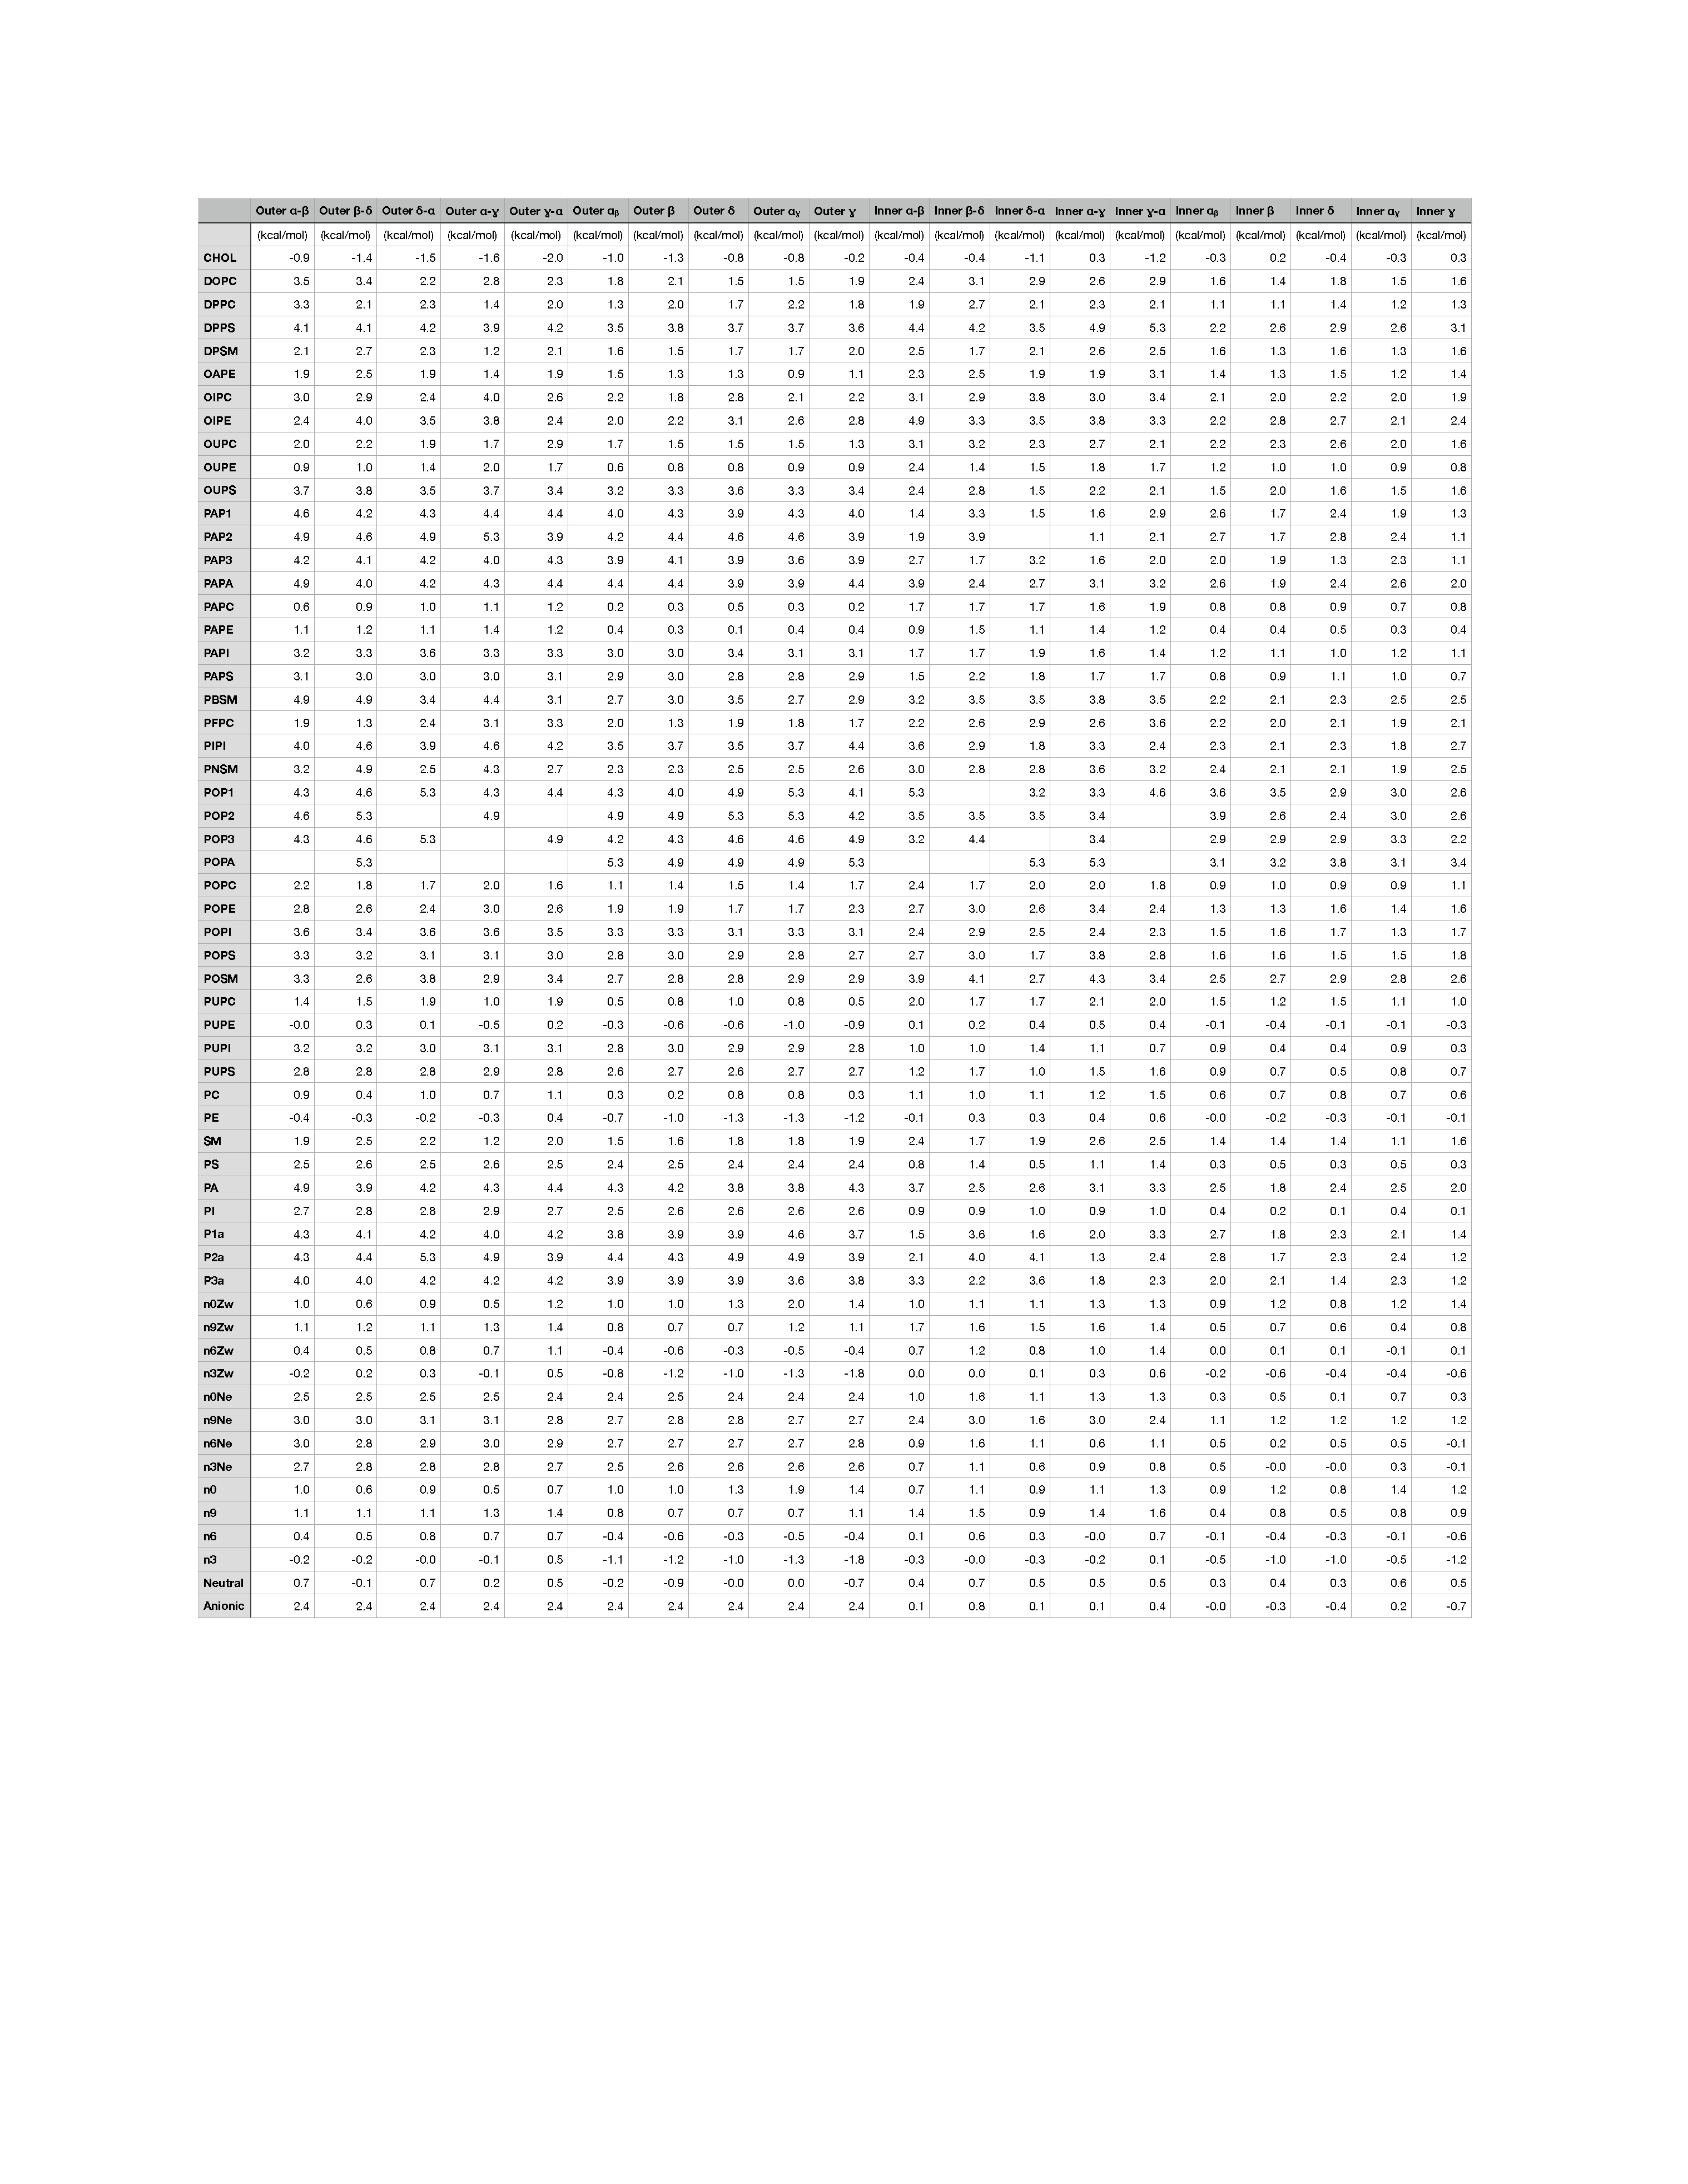
\includegraphics[width=\linewidth]{Full_dG.pdf}
%	\caption{$\Delta$G calculations for lipid spieces, head group, acyl-chain saturation, and charge.}
%	\label{fig:fullDG}
%\end{figure*}

%%
%% End of file `elsarticle-template-1-num.tex'.
